% Created 2019-12-18 Wed 15:41
% Intended LaTeX compiler: pdflatex
\documentclass[xcolor=table,10pt,aspectratio=169]{beamer}
\usepackage{graphicx}
\usepackage{grffile}
\usepackage{longtable}
\usepackage{wrapfig}
\usepackage{rotating}
\usepackage[normalem]{ulem}
\usepackage{amsmath}
\usepackage{textcomp}
\usepackage{amssymb}
\usepackage{capt-of}
\usepackage{hyperref}
\usepackage{microtype}
\usepackage{newunicodechar}
\usepackage[notions,operators,sets,keys,ff,adversary,primitives,complexity,asymptotics,lambda,landau,advantage]{cryptocode}
\usepackage{xspace}
\usepackage{units}
\usepackage{nicefrac}
\usepackage{gensymb}
\usepackage{amsthm}
\usepackage{amsmath}
\usepackage{amssymb}
\usepackage{xcolor}
\usepackage{listings}
\usepackage[color=yellow!40]{todonotes}
\RequirePackage{etex}
\RequirePackage[l2tabu,orthodox]{nag}            %% Warn about obsolete commands and packages
\RequirePackage{amsmath,amsfonts,amssymb,amsthm} %% Math
\RequirePackage{ifxetex,ifluatex}                %% Detect XeTeX and LuaTeX
\RequirePackage{fixltx2e}                        %% provides \textsubscript
\RequirePackage{xspace}
\RequirePackage{graphicx}
\RequirePackage{comment}
\RequirePackage{url}
\RequirePackage{relsize}
\RequirePackage{booktabs}
\RequirePackage{tabularx}
\RequirePackage[normalem]{ulem}
\RequirePackage[all]{xy}
\RequirePackage{etoolbox}

%%%
%%% Code Listings
%%%

\RequirePackage{listings}
\lstdefinelanguage{Sage}[]{Python}{morekeywords={True,False,sage,cdef,cpdef,ctypedef,self},sensitive=true}

\lstset{frame=none,
  showtabs=False,
  showspaces=False,
  showstringspaces=False,
  commentstyle={\color{gray}},
  keywordstyle={\color{mLightBrown}\textbf},
  stringstyle ={\color{mDarkBrown}},
  frame=single,
  basicstyle=\tt\scriptsize\relax,
  backgroundcolor=\color{gray!190!black},
  inputencoding=utf8,
  literate={…}{{\ldots}}1,
  belowskip=0.0em,
}

\makeatletter
\patchcmd{\@verbatim}
  {\verbatim@font}
  {\verbatim@font\scriptsize}
  {}{}
\makeatother

%%%
%%% Tikz
%%%

\RequirePackage{tikz,pgfplots}

\usetikzlibrary{calc}
\usetikzlibrary{arrows}
\usetikzlibrary{automata}
\usetikzlibrary{positioning}
\usetikzlibrary{decorations.pathmorphing}
\usetikzlibrary{backgrounds}
\usetikzlibrary{fit,}
\usetikzlibrary{shapes.symbols}
\usetikzlibrary{chains}
\usetikzlibrary{shapes.geometric}
\usetikzlibrary{shapes.arrows}
\usetikzlibrary{graphs}

%%%
%%% SVG (Inkscape)
%%%

\ifxetex % chktex 1
\newcommand{\executeiffilenewer}[3]{%
  {\immediate\write18{#3}} % hack
}
\else
\newcommand{\executeiffilenewer}[3]{%
  \ifnum\pdfstrcmp{\pdffilemoddate{#1}}%
    {\pdffilemoddate{#2}}>0%
    {\immediate\write18{#3}}
  \fi%
}
\fi

\newcommand{\includesvg}[2][1.0\textwidth]{%
 \executeiffilenewer{#1.svg}{#1.pdf}%
 {inkscape -z -D --file=#2.svg --export-pdf=#2.pdf --export-latex --export-area-page}%
 \def\svgwidth{#1} 
 \input{#2.pdf_tex}%
} 

%%%
%%% Metropolis Theme
%%%

\usetheme{metropolis}
\metroset{color/block=fill}
\metroset{numbering=none}
\metroset{outer/progressbar=foot}
\metroset{titleformat=smallcaps}

\setbeamercolor{description item}{fg=mLightBrown}
% \setbeamerfont{alerted text}{series=\bfseries}
\setbeamerfont{footnote}{size=\scriptsize}
\setbeamercolor{example text}{fg=mDarkBrown}
\setbeamercolor{block title alerted}{fg=white, bg=mDarkBrown}
\setbeamertemplate{bibliography item}[text]

\renewcommand*{\UrlFont}{\ttfamily\relax}

%%%
%%% UTF-8 & Fonts
%%% 

\RequirePackage{unicodesymbols} % after metropolis which loads fontspec

\setmonofont[BoldFont={Cousine Bold},
             ItalicFont={Cousine Italic},
             BoldItalicFont={Cousine Bold Italic},
             Scale=0.9]{Cousine}             
%%%
%%% BibLaTeX
%%%

\RequirePackage[backend=bibtex,
            style=alphabetic,
            maxnames=10,
            citestyle=alphabetic]{biblatex}

\bibliography{local.bib,abbrev3.bib,crypto_crossref.bib,rfc.bib,jacm.bib}

\DeclareFieldFormat{title}{\alert{#1}}
\DeclareFieldFormat[book]{title}{\alert{#1}}
\DeclareFieldFormat[thesis]{title}{\alert{#1}}
\DeclareFieldFormat[inproceedings]{title}{\alert{#1}}
\DeclareFieldFormat[incollection]{title}{\alert{#1}}
\DeclareFieldFormat[article]{title}{\alert{#1}}
\DeclareFieldFormat[misc]{title}{\alert{#1}}

%%% 
%%% Microtype
%%%

\IfFileExists{upquote.sty}{\RequirePackage{upquote}}{}
\IfFileExists{microtype.sty}{\RequirePackage{microtype}}{}

\setlength{\parindent}{0pt}                   %%
\setlength{\parskip}{6pt plus 2pt minus 1pt}  %%
\setlength{\emergencystretch}{3em}            %% prevent overfull lines
\setcounter{secnumdepth}{0}                   %%

\let\nl\undefine
\let\procedure\relax
\let\endprocedure\relax

\usepackage{algorithm2e}
\renewcommand{\vec}[1]{\mathbf{#1}\xspace}
\newcommand{\mat}[1]{\mathbf{#1}\xspace}

\definecolor{DarkPurple}{HTML}{332288}
\definecolor{DarkBlue}{HTML}{6699CC}
\definecolor{LightBlue}{HTML}{88CCEE}
\definecolor{DarkGreen}{HTML}{117733}
\definecolor{DarkRed}{HTML}{661100}
\definecolor{LightRed}{HTML}{CC6677}
\definecolor{LightPink}{HTML}{AA4466}
\definecolor{DarkPink}{HTML}{882255}
\definecolor{LightPurple}{HTML}{AA4499}
\definecolor{DarkBrown}{HTML}{604c38}
\definecolor{DarkTeal}{HTML}{23373b}
\definecolor{LightBrown}{HTML}{EB811B}
\definecolor{LightGreen}{HTML}{14B03D}
\definecolor{DarkOrange}{HTML}{FFDD00}

\pgfplotsset{width=1.0\textwidth,
  height=0.6\textwidth,
  xlabel={$\beta$},
  ylabel={$\log_{2}(\#\textnormal{nodes})$},
  cycle list={%
    solid,LightGreen,thick\\%
    dotted,LightRed,very thick\\%
    dashed,DarkBlue,thick\\%
    dashdotted,DarkPink,thick\\%
    dashdotdotted,LightGreen,thick\\%
    loosely dotted,very thick\\%
    loosely dashed,DarkBlue,very thick\\%
    loosely dashdotted,DarkPink,very thick\\%
    \\%
    DarkBrown,thick\\%
  },
  legend pos=north west,
  legend cell align={left}}

\pgfplotsset{select coords between index/.style 2 args={
    x filter/.code={
        \ifnum\coordindex<#1\def\pgfmathresult{}\fi
        \ifnum\coordindex>#2\def\pgfmathresult{}\fi
    }
}}


%%% Local Variables:
%%% mode: latex
%%% End:
\def\enumworstfit{\(1/(2e)\, \beta \log(\beta) - \beta + 16.1\)}
\def\enumavgfit{\(1/8\,\beta \log(\beta) - 0.75\beta + 2.3\)}
\def\qenumworstfit{\(1/(4e)\, \beta \log(\beta) - 1/2\beta + 8\)}
\def\robl{\rowcolor{DarkBlue!20}}
\def\rore{\rowcolor{DarkRed!20}}
\def\rogr{\rowcolor{gray!20}}
\usetheme{default}
\author{Martin R. Albrecht \alert{@martinralbrecht}}
\date{10 July 2019, AfricaCrypt\vfill \begin{scriptsize}Based on joint work with Alex Davidson, Amit Deo, Benjamin R. Curtis, Eamonn W. Postlethwaite, Elena Kirshanova, Fernando Virdia, Florian Göpfert, Gottfried Herold, John M. Schanck, Léo Ducas, Marc Stevens, Rachel Player, Sam Scott, Thomas Wunderer and Vlad Gheorghiu as well as the work of many other authors.\end{scriptsize}}
\title{So how hard is solving hard lattice problems anyway?}
\hypersetup{
pdfauthor={Martin R. Albrecht \alert{@martinralbrecht}},
pdftitle={So how hard is solving hard lattice problems anyway?},
pdfkeywords={},
pdfsubject={},
pdfcreator={Emacs 26.3 (Org mode 9.3)},
pdflang={English},
colorlinks,
citecolor=gray,
filecolor=gray,
linkcolor=gray,
urlcolor=gray
}
\begin{document}

\maketitle

\section{Introduction}
\label{sec:org6105e26}
\begin{frame}[label={sec:org47f5f41}]{NIST Round 1: Selected Cost Estimates}
\rowcolors[]{3}{gray!20}{gray!10}

\begin{center}
\small{
\begin{tabular}{rrrrr}
\textbf{Cost Model} $\backslash$    \textbf{Scheme} & \textbf{Kyber} & \textbf{NewHope} & \textbf{NTRU HRSS} & \textbf{SNTRU'}\\
\hline
\(0.292\,β\)\footnotemark & 180 & 259 & 136 & 155\\
\enumworstfit \footnotemark & 456 & 738 & 313 & 370\\
\enumavgfit \footnotemark & 248 & 416 & 165 & 200\\
\hline
\(0.265\,\beta\)\textsuperscript{\ref{orgf3aa08e}} & 163 & 235 & 123 & 140\\
\qenumworstfit & 228 & 369 & 157 & 187\\
\end{tabular}
\footnotetext[1]{\label{orgf3aa08e}\fullcite{USENIX:ADPS16}}\footnotetext[2]{\label{org0b6d635}\fullcite{JMC:AlbPlaSco15}}\footnotetext[3]{\label{org6f64db5}\fullcite{NISTPQC-R1:LOTUS17}}
}
\end{center}

\scriptsize{
Source: \fullcite{SCN:ACDDPP18}, \url{https://estimate-all-the-lwe-ntru-schemes.github.io/docs/}
}

\vspace{1em}
\end{frame}

\begin{frame}[label={sec:org0bae23b}]{Learning with Errors}
Given \((\mathbf{A},\vec{c})\), find \(\vec{s}\) when

\[
\left(\begin{array}{c}
\\
\\
\\ 
\vec{c} \\
\\
\\
\\
\end{array} \right) \equiv \left(
\begin{array}{ccc}
\leftarrow & n & \rightarrow \\
\\
\\ 
& \mathbf{A} & \\
\\
\\
\\
\end{array} \right) \cdot \left( \begin{array}{c}
\\\
\\
\vec{s} \\
\\
\\
\end{array} \right) + \left(
\begin{array}{c}
\\
\\
\\ 
\vec{e} \\
\\
\\
\\
\end{array} 
\right)
\]

for \(\vec{c} \in \ZZ_q^{m}\), \(\mathbf{A} \in \ZZ_q^{m \times n}\), and \(\vec{s} \in \ZZ^{n}\) and \(\vec{e} \in \ZZ^{m}\) having small coefficients.
\end{frame}

\begin{frame}[label={sec:org3197975}]{(Matrix-)NTRU}
Let \(\mathbf{F}, \mathbf{G}\) be two \(n \times n\) matrices over \(\ZZ_q\) with short entries. Given
\[\mathbf{H} \equiv \mathbf{F}^{-1} \cdot \mathbf{G}\]
find (a small multiple of) \(\mathbf{F}\) or \(\mathbf{G}\).

\pause

\begin{block}{Note}
I will focus on LWE in this talk, but the techniques translate (with some modifications) to NTRU.
\end{block}
\end{frame}

\section{Primal Approach}
\label{sec:orga734c62}
\begin{frame}[label={sec:orge1309da}]{Unique SVP Approach}
We can reformulate \(\vec{c} - \mathbf{A} \cdot \vec{s} \equiv \vec{e} \bmod q\)  over the Integers as:
\[
  \begin{pmatrix}
    q\mathbf{I} & -\mathbf{A}\\
    0 & \mathbf{I}\\
  \end{pmatrix} \cdot
  \begin{pmatrix}
    \mathbf{*}\\
    \mathbf{s}
  \end{pmatrix} +
  \begin{pmatrix}
    \vec{c}\\
    \vec{0}
  \end{pmatrix} = 
  \begin{pmatrix}
    \vec{e}\\
    \vec{s}
  \end{pmatrix}
\]
Alternatively:
\[
  \mathbf{B} = \begin{pmatrix}
    q\mathbf{I} & -\mathbf{A} & \vec{c}\\
    0 & \mathbf{I} & 0\\
    0 & 0 & 1\\
  \end{pmatrix}, \qquad
  \mathbf{B} \cdot
  \begin{pmatrix}
    \vec{*}\\
    \vec{s}\\
    1
  \end{pmatrix} = 
  \begin{pmatrix}
    \vec{e}\\
    \vec{s}\\
    1
  \end{pmatrix}
\]

In other words, there exists an integer-linear combination of the columns of \(\mathbf{B}\) that produces a vector with “unusually” small coefficients \(\rightarrow\) a unique shortest vector.
\end{frame}

\begin{frame}[label={sec:orge896f7c}]{Computational Problem}
\begin{block}{Unique Shortest Vector Problem}
Find a unique shortest vector amongst the integer combinations of the columns of:
\[
  \mathbf{B} = \begin{pmatrix}
    q\mathbf{I} & -\mathbf{A} & \vec{c}\\
    0 & \mathbf{I} & 0\\
    0 & 0 & 1\\
  \end{pmatrix}
\]
where \(\mat{B} \in \ZZ^{d \times d}\).

\pause
\end{block}

\begin{alertblock}{NTRU}
In the case of LWE we have (up to \(\pm\)) one such short vector. In the case of NTRU we have \(n\).
\end{alertblock}
\end{frame}

\section{Lattice Reduction}
\label{sec:org39254a9}
\begin{frame}[label={sec:org52bcfb9}]{Lattices}
A lattice is a discrete subgroup of \(\mathbb{R}^d\) and can be written as \(\Lambda = \{\sum_{i=1}^{d} v_i \cdot \vec{b}_i \mid v_i \in \ZZ\}\)

\begin{center}
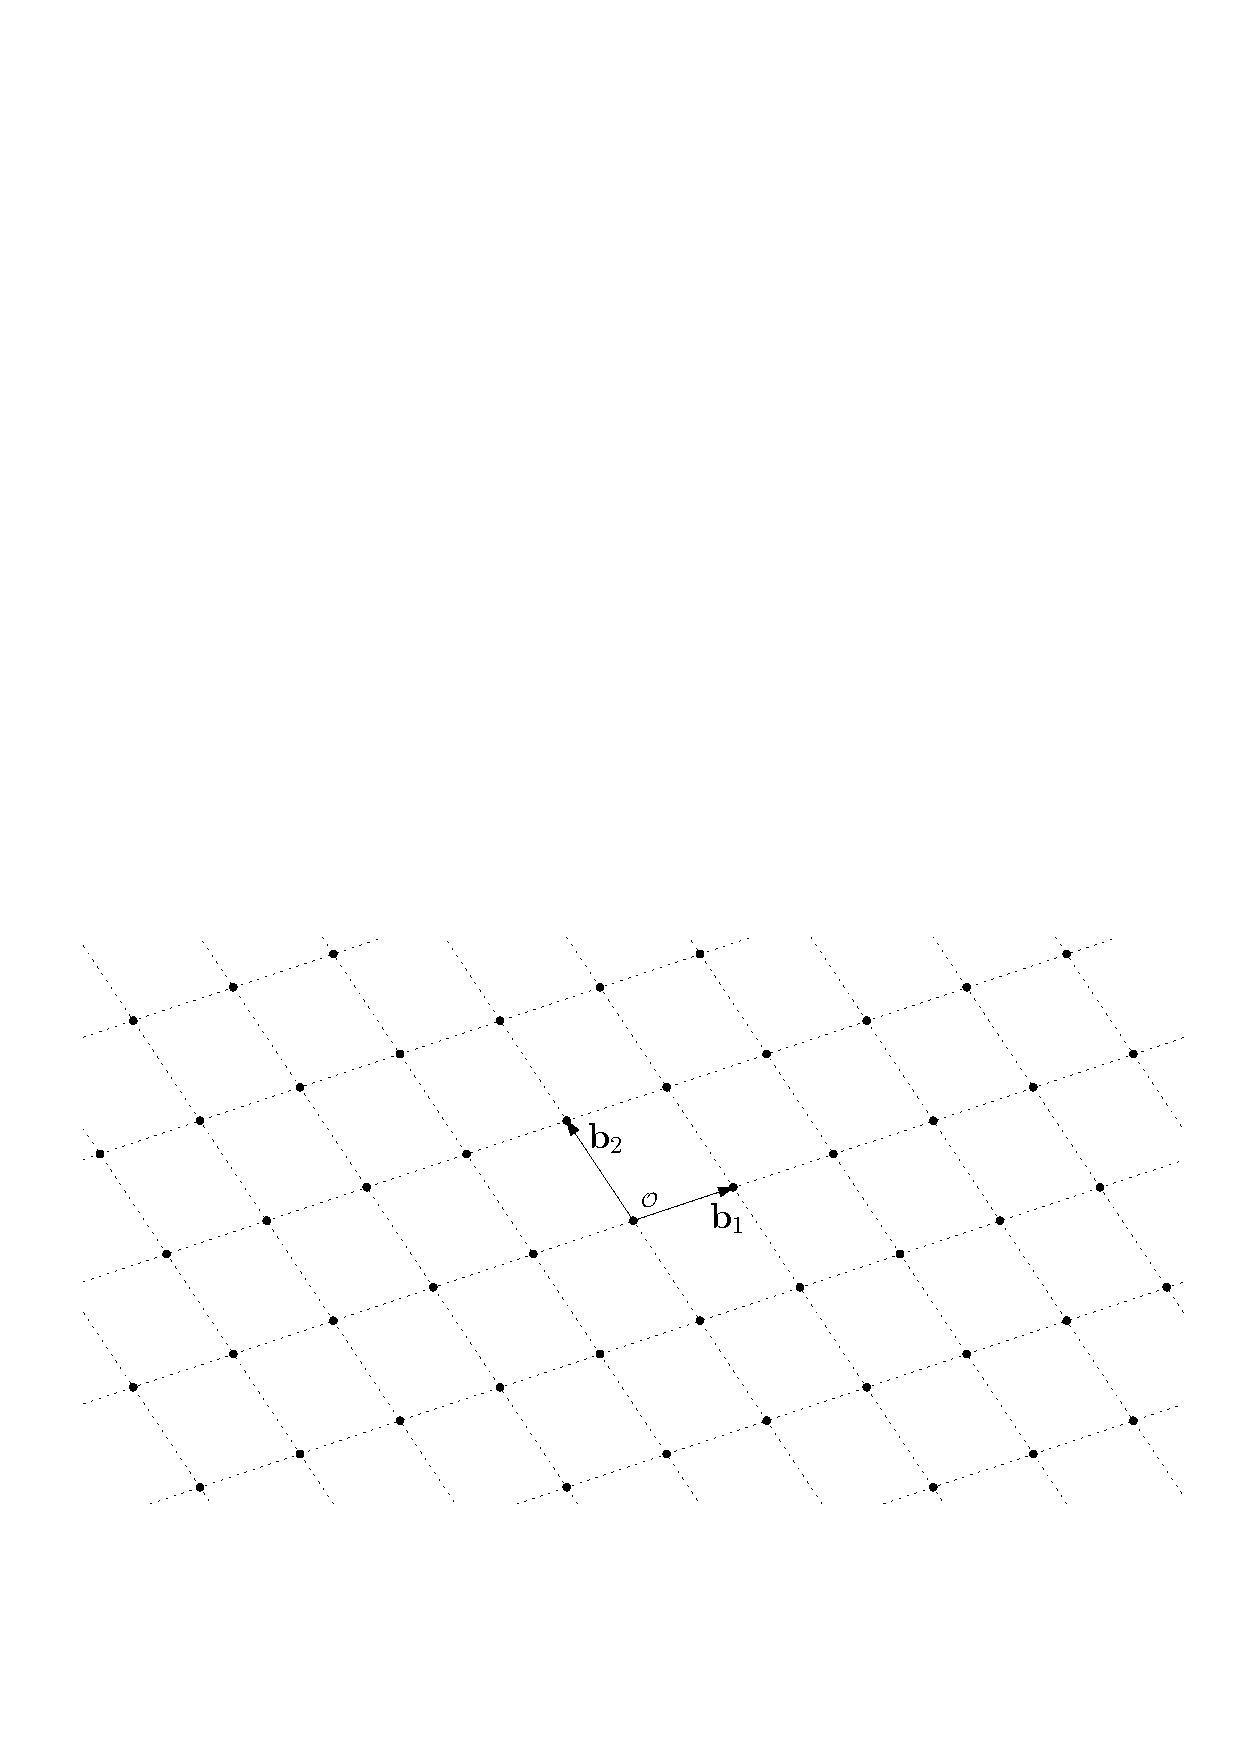
\includegraphics[width=0.8\linewidth]{./joop-latt1.pdf}
\end{center}

\tiny Picture Credit: Joop van de Pol
\end{frame}

\begin{frame}[label={sec:orgdb8c34e}]{A Tale of Bad Bases …}
With “bad basis” finding short vectors assumed hard.

\begin{center}
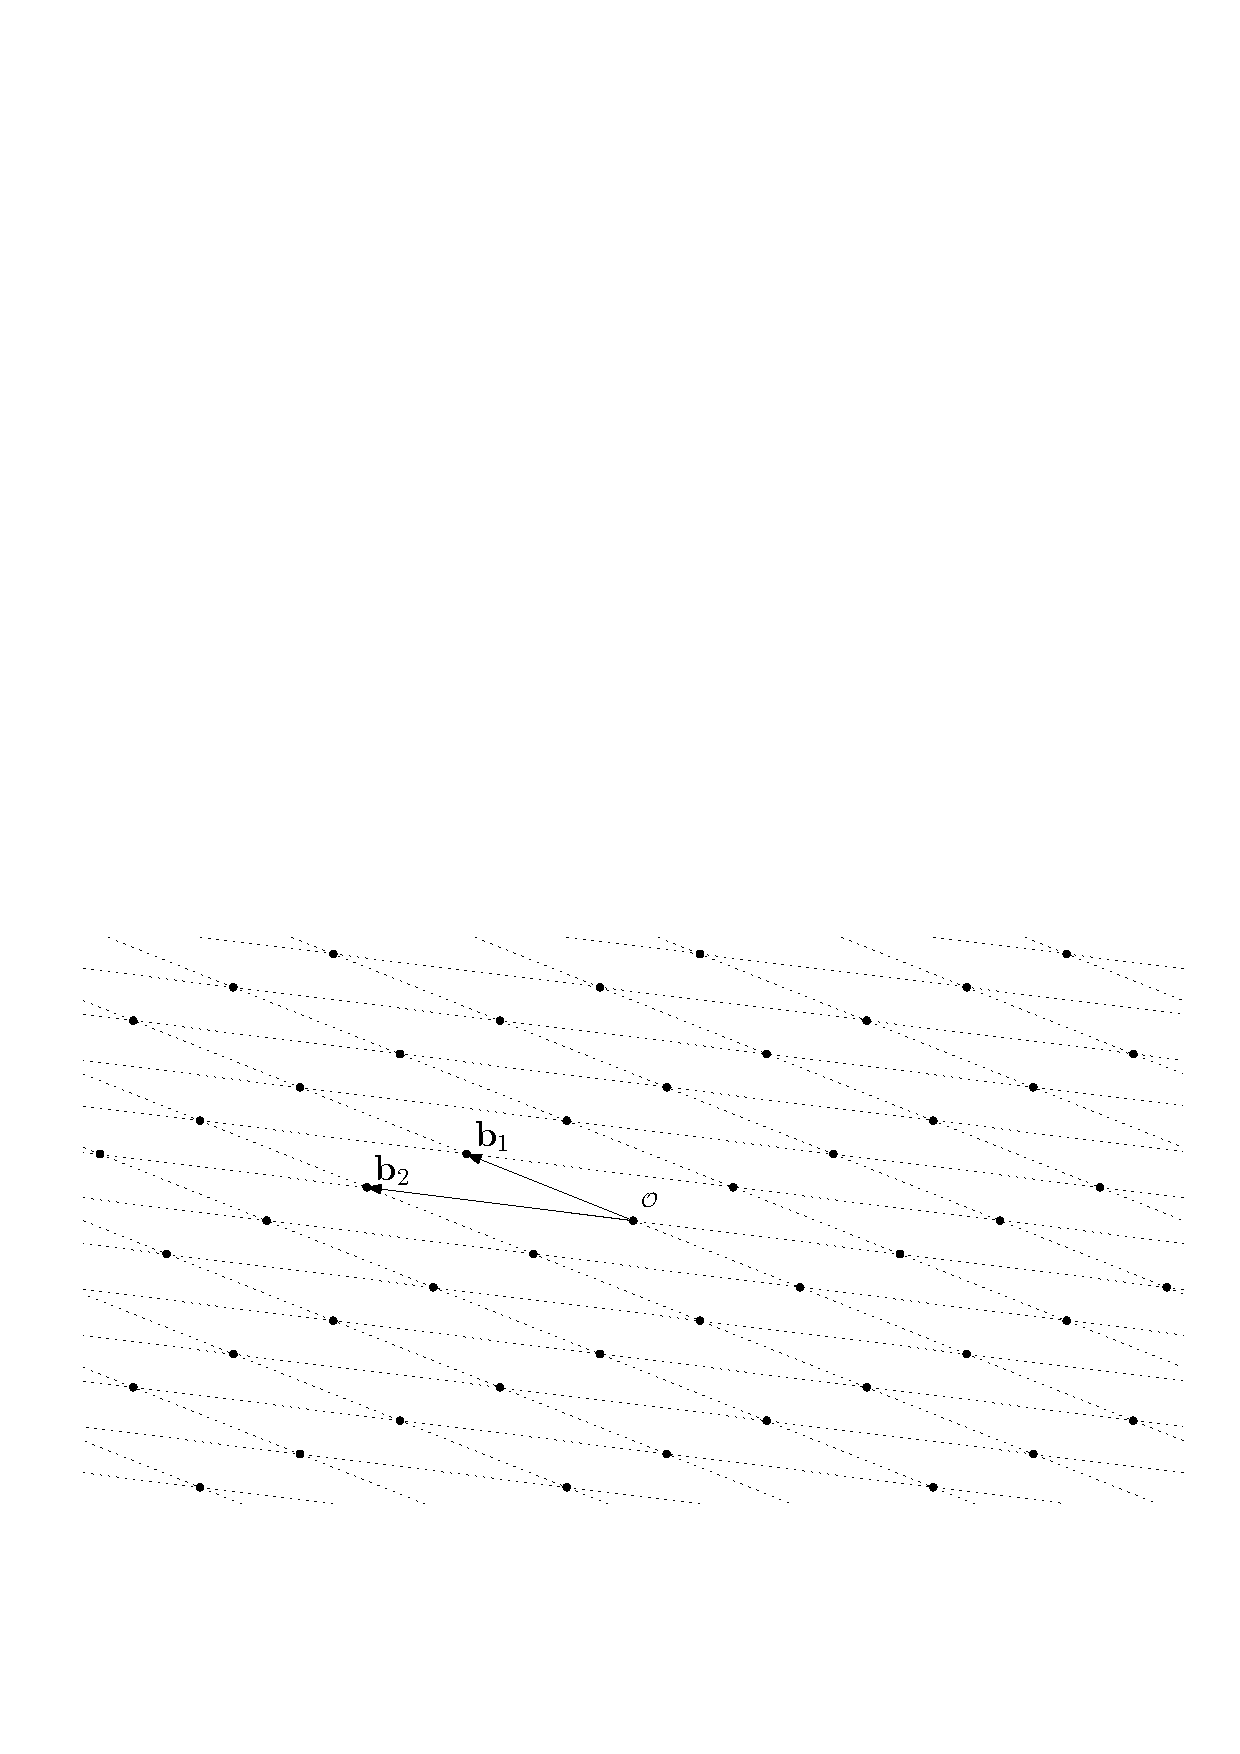
\includegraphics[width=0.8\linewidth]{./joop-latt2a.pdf}
\end{center}

\tiny Picture Credit: Joop van de Pol
\end{frame}

\begin{frame}[label={sec:org158f189}]{… and Good Bases}
With a “good basis” many lattice problems are easy.

\begin{center}
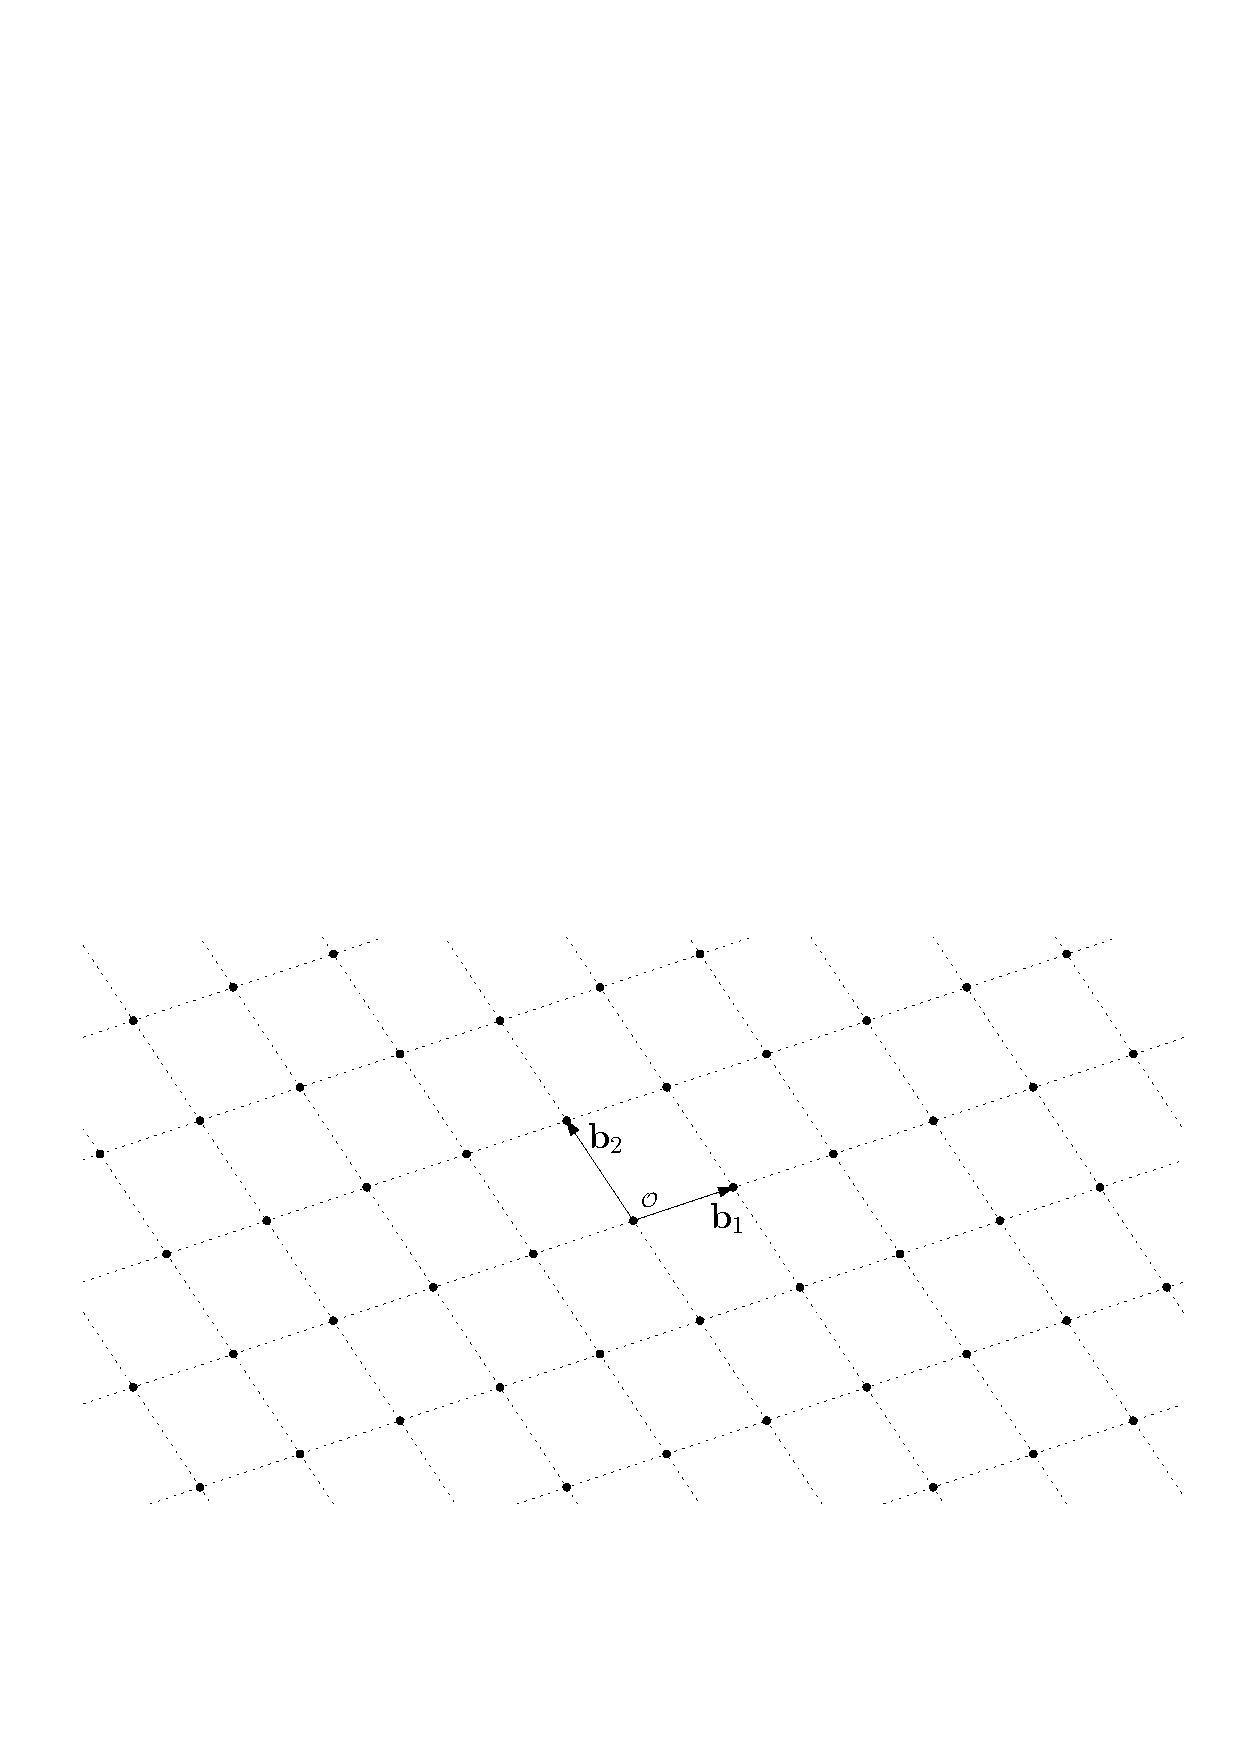
\includegraphics[width=0.8\linewidth]{./joop-latt1.pdf}
\end{center}

\tiny Picture Credit: Joop van de Pol
\end{frame}

\begin{frame}[label={sec:org782d688}]{Lattice Volume}
The volume of a lattice is the volume of its fundamental parallelepiped.

\begin{center}
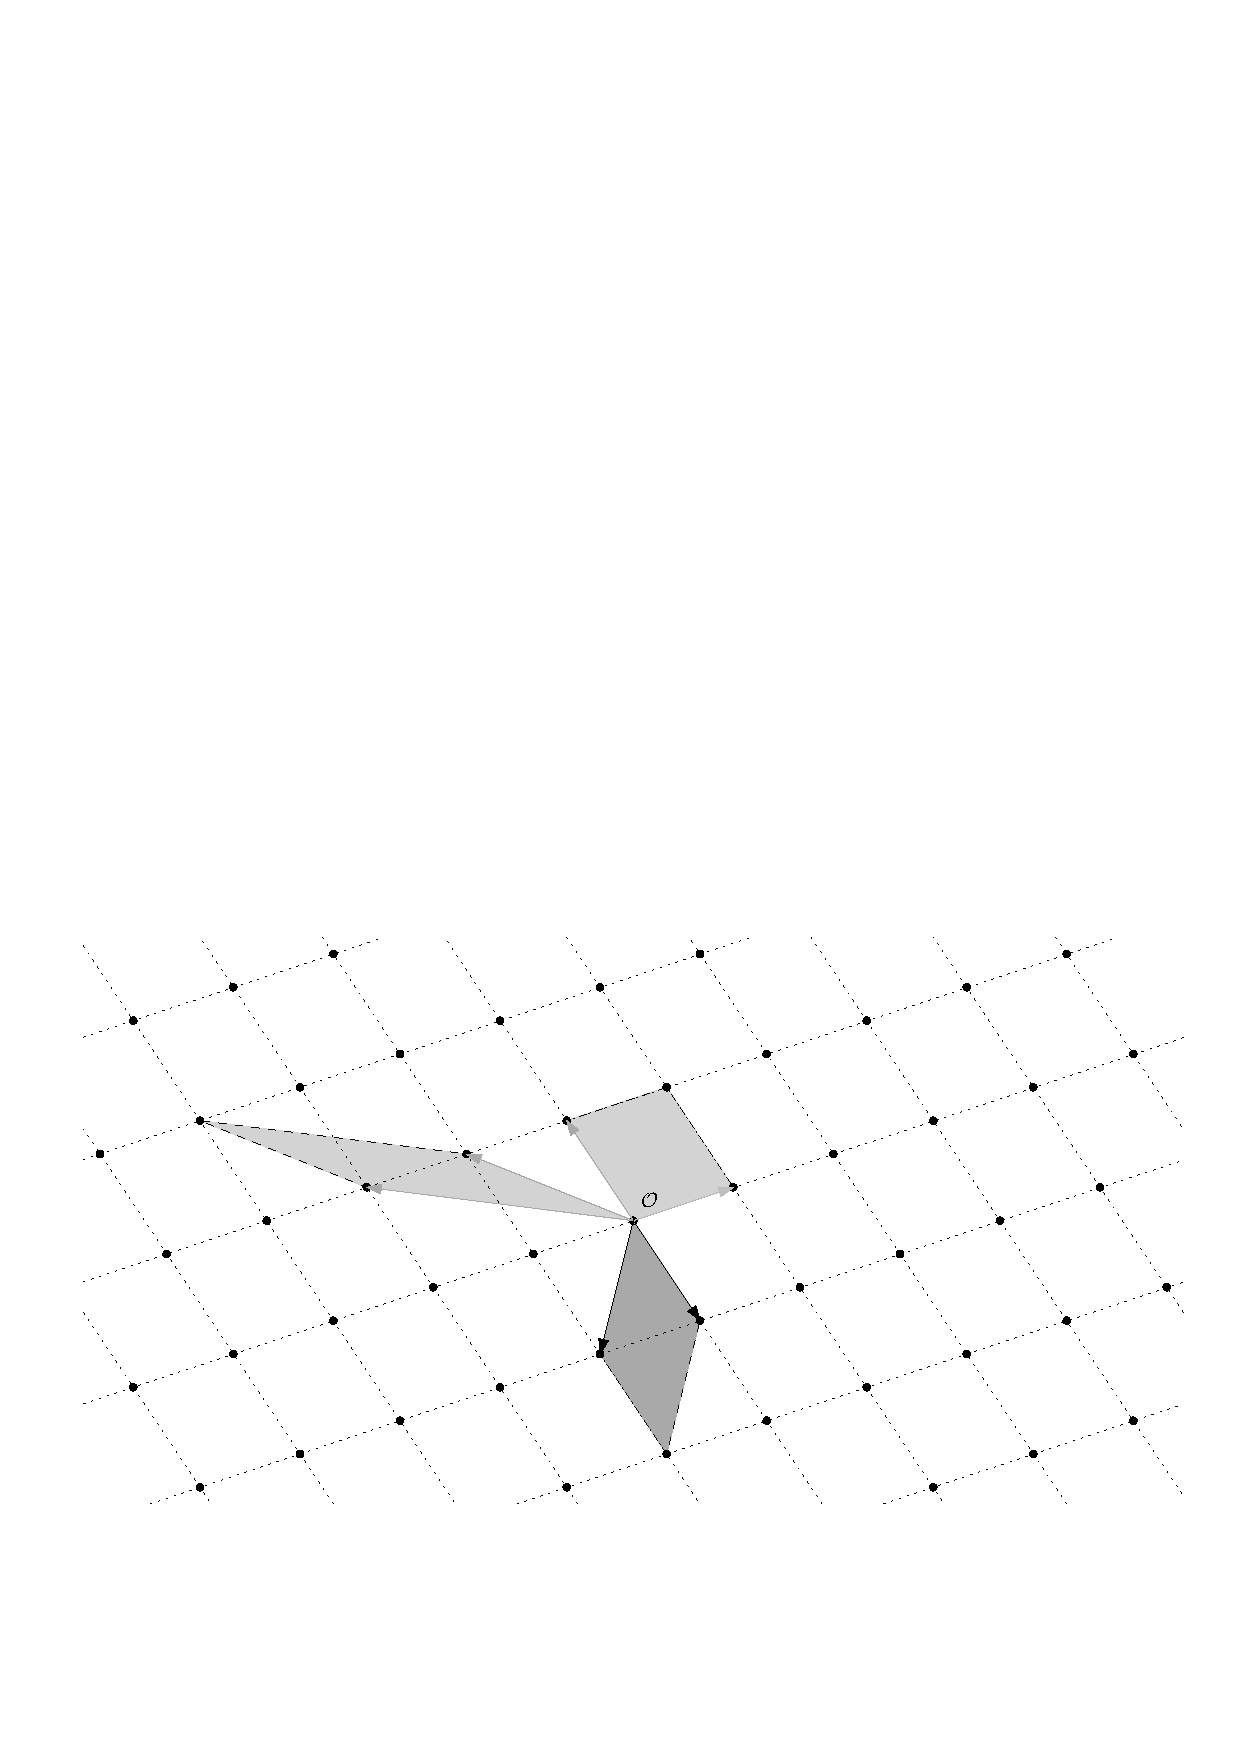
\includegraphics[width=0.8\linewidth]{./joop-vol3.pdf}
\end{center}

\tiny Picture Credit: Joop van de Pol
\end{frame}

\begin{frame}[label={sec:orga6a0826}]{Gaussian Heuristic}
The shortest vector in the lattice has expected norm \[λ_1(Λ) ≈ \sqrt{\frac{d}{2 π e}} \mathsf{Vol}(\Lambda)^{1/d}.\]

\begin{block}{Unusually Shortest Vector}
When \(λ_1(Λ) \ll \sqrt{\frac{d}{2 π e}} \mathsf{Vol}(\Lambda)^{1/d}\).
\end{block}
\end{frame}

\begin{frame}[label={sec:org830a9b2}]{Length of Gram-Schmidt Vectors}
It will be useful to consider the lengths of the Gram-Schmidt vectors.

The vector \(\vec{b}^*_i\) is the orthogonal projection of \(\vec{b}_i\) to the space spanned by the vectors \(\vec{b}_0, \ldots, \vec{b}_{i-1}\).

\begin{columns}
\begin{column}{0.45\columnwidth}
Informally, this means taking out the contributions in the directions of previous vectors  \(\vec{b}_0, \ldots, \vec{b}_{i-1}\).
\end{column}

\begin{column}{0.45\columnwidth}
\begin{tikzpicture}
\pgfplotsset{width=\textwidth, height=0.6\textwidth}
\draw[->] (0,0) -- (3,1);
\node[] at (3.2,1.2) {$\vec{b}_0$};
\only<1>{\draw[->] (0,0) -- (1,2);}
\only<1>{\node[] at (1.2,2.2) {$\vec{b}_1$};}
\only<2>{\draw[->,color=lightgray] (0,0) -- (1,2);}
\only<2>{\node[color=lightgray] at (1.2,2.2) {$\vec{b}_1$};}
\only<2>{\draw[->,gray] (0,0) -- (-0.5,1.5);}
\only<2>{\node[] at (-0.3,1.7) {$\vec{b}^*_1$};}
\only<1>{\node[] at (-0.3,1.7) {\phantom{$\vec{b}^*_1$}};}
\end{tikzpicture}
\end{column}
\end{columns}
\end{frame}

\begin{frame}[label={sec:orgeadea81},fragile]{Example}
 \lstset{language=sage,label= ,caption= ,captionpos=b,numbers=none}
\begin{lstlisting}
sage: A = IntegerMatrix.random(120, "qary", k=60, bits=20)[::-1]
sage: M = GSO.Mat(A); M.update_gso()
sage: lg = [(i,log(r_, 2)/2) for i, r_ in enumerate(M.r())]
sage: line(lg, **plot_kwds)
\end{lstlisting}

\begin{center}
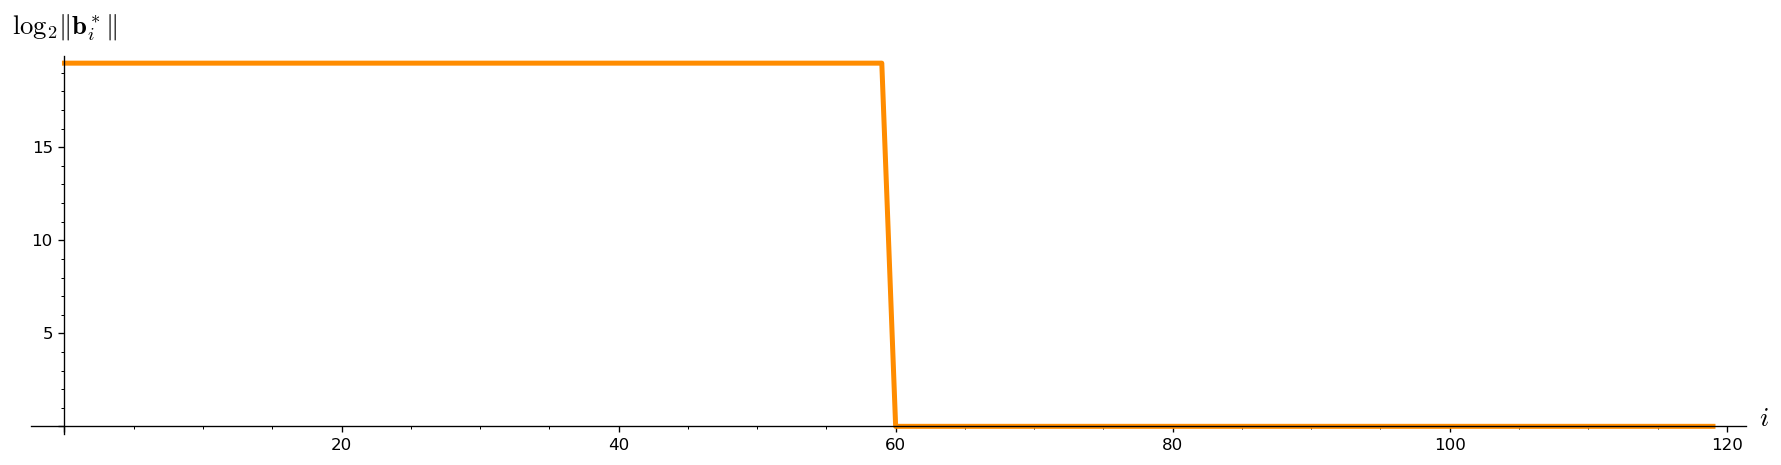
\includegraphics[width=.9\linewidth]{gram-schmidt-norms.png}
\end{center}
\end{frame}

\begin{frame}[label={sec:org31e0df5},fragile]{Example - LLL}
 \lstset{language=sage,label= ,caption= ,captionpos=b,numbers=none}
\begin{lstlisting}
sage: A = LLL.reduction(A)
sage: M = GSO.Mat(A); M.update_gso()
sage: lg = [(i,log(r_, 2)/2) for i, r_ in enumerate(M.r())]
sage: line(lg, **plot_kwds)
\end{lstlisting}

\begin{center}
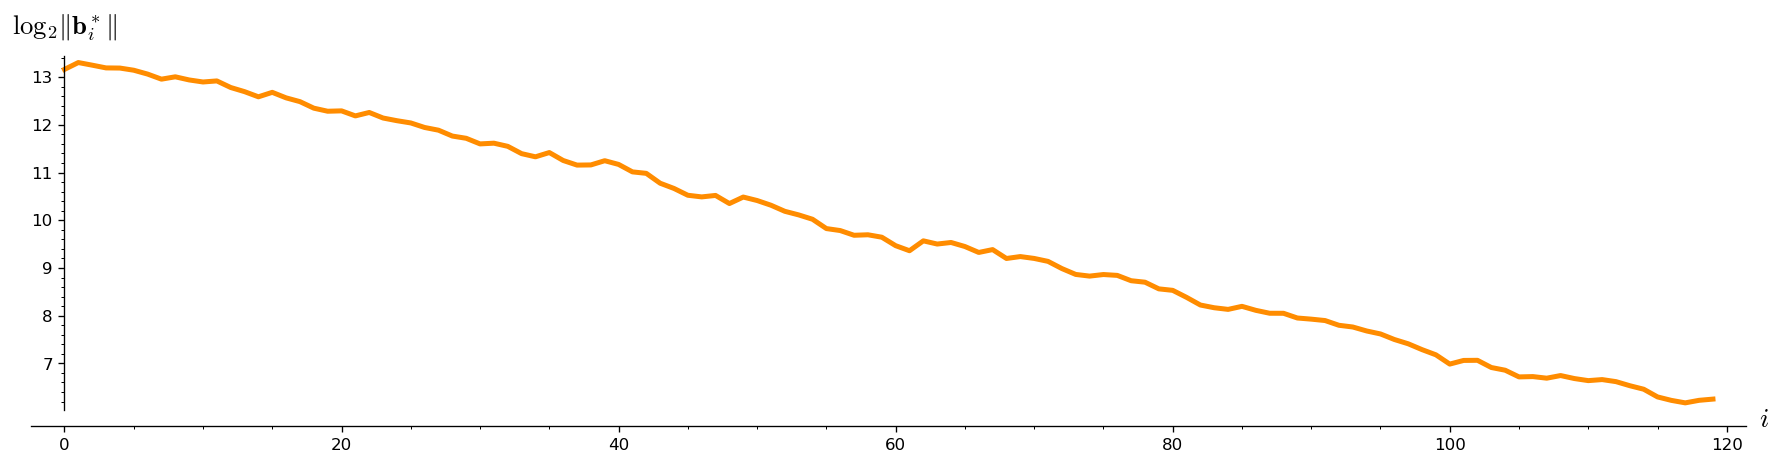
\includegraphics[width=.9\linewidth]{gram-schmidt-norms-lll.png}
\end{center}

\textbf{Geometric Series Assumption:} The shape after lattice reduction is a line with a flatter slope as lattice reduction gets stronger.
\end{frame}

\begin{frame}[label={sec:org0df4c41}]{Strong Lattice Reduction: BKZ Algorithm}
\centering
\(
 \left(
     \begin{array}{ccccccccc}
                 &           &           &           &           &           &           &           &           \\
                 &           &           &           &           &           &           &           &           \\
                 &           &           &           &           &           &           &           &           \\
         \only<1-2>{\vec{b}_{0}}   \only<3->{{\color{LightRed} \vec{b}_{0}}}          &
         \only<1-5>{\vec{b}_{1}}   \only<6->{{\color{LightRed} \vec{b}_{1}}}          &
         \only<1-8>{\vec{b}_{2}}   \only<9->{{\color{LightRed} \vec{b}_{2}}}          &
         {\vec{b}_{3}}                                                             &
         {\vec{b}_{4}}                                                             &
         {\vec{b}_{5}}                                                             &
         {\vec{b}_{6}}                                                             &
         {\vec{b}_{7}}                                                             &
         \dots   \\
                 &           &           &           &           &           &           &           &           \\
                 &           &           &           &           &           &           &           &           \\
                 &           &           &           &           &           &           &           &
     \end{array}
        \right)
    \)
    \begin{tikzpicture}[remember picture, overlay]
      \tikzset{shift={(current page.center)},yshift=-1.5cm}
      \node[] at (0,0) (origin) {};
      {\color{DarkBlue} %
        \only<1-3>{%
          \draw (-.1,3) -- (-.1,2) {};
          \draw (-.1,1) -- (-.1,0) {};
          \draw (-3,3) -- (-3,2) {};
          \draw (-3,1) -- (-3,0) {};
          \draw[decorate,decoration={brace,amplitude=10pt}]
          (-3,3.2) -- (-.1,3.2) node [black,midway,yshift=.6cm]
          {$\beta = 5$};
          \only<2>{%
            \draw[decorate,decoration={brace,amplitude=10pt}]
            (-.1,-.2) -- (-3,-.2) {};
          }
        }
        \only<4-6>{%
          \draw (.6,3) -- (.6,2) {};
          \draw (.6,1) -- (.6,0) {};
          \draw (-2.3,3) -- (-2.3,2) {};
          \draw (-2.3,1) -- (-2.3,0) {};
          \draw[decorate,decoration={brace,amplitude=10pt}]
          (-2.3,3.2) -- (.6,3.2) node [black,midway,yshift=.6cm]
          {$\beta = 5$};
          \only<5>{%
            \draw[decorate,decoration={brace,amplitude=10pt}]
            (.6,-.2) -- (-2.3,-.2) {};
          }
        }
        \only<7-9>{%
          \draw (1.3,3) -- (1.3,2) {};
          \draw (1.3,1) -- (1.3,0) {};
          \draw (-1.6,3) -- (-1.6,2) {};
          \draw (-1.6,1) -- (-1.6,0) {};
          \draw[decorate,decoration={brace,amplitude=10pt}]
          (-1.6,3.2) -- (1.3,3.2) node [black,midway,yshift=.6cm]
          {$\beta = 5$};
          \only<8>{%
            \draw[decorate,decoration={brace,amplitude=10pt}]
            (1.3,-.2) -- (-1.6,-.2) {};
          }
        }
      }
      \node (oracle) at (-4,-1.8) {
\includegraphics[scale=0.9]{oracle.png}};
      \only<2>{%
        \draw[->] (-2.8,-.5) to[in=70,out=160] (-4,-.8);
        \draw[->] (-3,-2) to [in=270,out=20] (-0.5,-.5);
      }
      \only<5>{%
        \draw[->] (-2.1,-.5) to[in=70,out=160] (-4,-.8);
        \draw[->] (-3,-2) to [in=270,out=20] (.2,-.5);
      }
      \only<8>{%
        \draw[->] (-1.4,-.5) to[in=70,out=160] (-4,-.8);
        \draw[->] (-3,-2) to [in=270,out=20] (.2,-.5);      
      }
      \node at (5, -2.5) {\tiny{Picture credit: Eamonn Postlethwaite}};
\end{tikzpicture}
\end{frame}

\begin{frame}[label={sec:org3edc34d}]{BKZ Algorithm}
\begin{algorithm}[H]
  \KwData{LLL-reduced lattice basis \(\mat{B}\)}
  \KwData{block size \(\beta\)}
  \SetKwFor{MRepeat}{repeat}{}{}
  \MRepeat{until no more change}{
    \For{\(\kappa \gets 0\) \KwTo{} \(d-1\)}{
        LLL  on local projected block \([\kappa,\ldots,\kappa+\beta-1]\)\; 
        \(\vec{v} \gets \) find shortest vector in local projected block \([\kappa,\ldots,\kappa+\beta-1]\)\;
        insert $\vec{v}$ into $\vec{B}$\;
    }
  }
\end{algorithm}

\begin{block}{Jargon}
An outer loop iteration is called a “tour”.
\end{block}
\end{frame}
\begin{frame}[label={sec:org368d4a7}]{Slope}
The slope depends on the \textbf{root Hermite factor} \(\delta\) which depends on the block size \(\beta\).

\tikzset{external/export=true}
\tikzsetnextfilename{root-hermite-factor}
\begin{tikzpicture}
\pgfplotsset{width=\textwidth, height=0.4\textwidth}

\begin{axis}[xlabel={$\beta$},ylabel={$\delta$},legend pos=north east, legend style={fill=none},  yticklabel style={/pgf/number format/fixed, /pgf/number format/precision=4}]
         	
\addplot[black, thick] coordinates {
(50, 1.01206486355485) (60, 1.01145310214785) (70, 1.01083849117278)
(80, 1.01026264533039) (90, 1.00973613406057) (100, 1.00925872103633)
(110, 1.00882653150498) (120, 1.00843474281592) (130, 1.00807860284815)
(140, 1.00775378902354) (150, 1.00745650119215) (160, 1.00718344897388)
(170, 1.00693180103572) (180, 1.00669912477197) (190, 1.00648332800111)
(200, 1.00628260691082) (210, 1.00609540127612) (220, 1.00592035664374)
(230, 1.00575629268952) (240, 1.00560217684407) (250, 1.00545710232739)
};
\addlegendentry{$(\frac{\beta}{2\pi e} \cdot (\pi\, \beta)^{1/\beta} )^{\frac{1}{2(\beta-1)}}$};

\end{axis}
\end{tikzpicture}
\tikzset{external/export=false}

\small{

\fullcite{PhD:Chen13}

}
\end{frame}

\begin{frame}[allowframebreaks]{Behaviour in Practice: BKZ-60 in Dimension 180}
\tikzset{external/export=true}

\vspace{-0.8em}
\tikzsetnextfilename{bkz-behaviour-0-lll}
\begin{tikzpicture}
  \begin{axis}[ylabel=\(\log_2(\|\vec{b}_i^*\|)\),xlabel=\(i\),legend pos=north east,height=0.5\textwidth,ymin=3,ymax=16,xmin=0,xmax=180]
    \addplot+[black] table [x=i, y=gsa, col sep=comma]{data/bkz-60-180.csv};
    \addlegendentry{GSA};
    \addplot+[] table [x=i, y=lll, col sep=comma]{data/bkz-60-180.csv};
    \addlegendentry{LLL};
  \end{axis}
\end{tikzpicture}

\framebreak

\tikzsetnextfilename{bkz-behaviour-1}
\begin{tikzpicture}
  \begin{axis}[ylabel=\(\log_2(\|\vec{b}_i^*\|)\),xlabel=\(i\),legend pos=north east,height=0.5\textwidth,ymin=3,ymax=16,xmin=0,xmax=180]
    \addplot+[black] table [x=i, y=gsa, col sep=comma]{data/bkz-60-180.csv};
    \addlegendentry{GSA};
    \addplot+[] table [x=i, y=tour0, col sep=comma]{data/bkz-60-180.csv};
    \addlegendentry{Tour 0};
  \end{axis}
\end{tikzpicture}

\framebreak

\tikzsetnextfilename{bkz-behaviour-2}
\begin{tikzpicture}
  \begin{axis}[ylabel=\(\log_2(\|\vec{b}_i^*\|)\),xlabel=\(i\),legend pos=north east,height=0.5\textwidth,ymin=3,ymax=16,xmin=0,xmax=180]
    \addplot+[black] table [x=i, y=gsa, col sep=comma]{data/bkz-60-180.csv};
    \addlegendentry{GSA};
    \addplot+[] table [x=i, y=tour1, col sep=comma]{data/bkz-60-180.csv};
    \addlegendentry{Tour 1};
  \end{axis}
\end{tikzpicture}


\framebreak

\tikzsetnextfilename{bkz-behaviour-3}
\begin{tikzpicture}
  \begin{axis}[ylabel=\(\log_2(\|\vec{b}_i^*\|)\),xlabel=\(i\),legend pos=north east,height=0.5\textwidth,ymin=3,ymax=16,xmin=0,xmax=180]
    \addplot+[black] table [x=i, y=gsa, col sep=comma]{data/bkz-60-180.csv};
    \addlegendentry{GSA};
    \addplot+[] table [x=i, y=tour2, col sep=comma]{data/bkz-60-180.csv};
    \addlegendentry{Tour 2};
  \end{axis}
\end{tikzpicture}

\framebreak

\tikzsetnextfilename{bkz-behaviour-4}
\begin{tikzpicture}
  \begin{axis}[ylabel=\(\log_2(\|\vec{b}_i^*\|)\),xlabel=\(i\),legend pos=north east,height=0.5\textwidth,ymin=3,ymax=16,xmin=0,xmax=180]
    \addplot+[black] table [x=i, y=gsa, col sep=comma]{data/bkz-60-180.csv};
    \addlegendentry{GSA};
    \addplot+[] table [x=i, y=tour3, col sep=comma]{data/bkz-60-180.csv};
    \addlegendentry{Tour 3};
  \end{axis}
\end{tikzpicture}

\framebreak

\tikzsetnextfilename{bkz-behaviour-5}
\begin{tikzpicture}
  \begin{axis}[ylabel=\(\log_2(\|\vec{b}_i^*\|)\),xlabel=\(i\),legend pos=north east,height=0.5\textwidth,ymin=3,ymax=16,xmin=0,xmax=180]
    \addplot+[black] table [x=i, y=gsa, col sep=comma]{data/bkz-60-180.csv};
    \addlegendentry{GSA};
    \addplot+[] table [x=i, y=tour4, col sep=comma]{data/bkz-60-180.csv};
    \addlegendentry{Tour 4};
  \end{axis}
\end{tikzpicture}

\framebreak

\tikzsetnextfilename{bkz-behaviour-6}
\begin{tikzpicture}
  \begin{axis}[ylabel=\(\log_2(\|\vec{b}_i^*\|)\),xlabel=\(i\),legend pos=north east,height=0.5\textwidth,ymin=3,ymax=16,xmin=0,xmax=180]
    \addplot+[black] table [x=i, y=gsa, col sep=comma]{data/bkz-60-180.csv};
    \addlegendentry{GSA};
    \addplot+[] table [x=i, y=tour5, col sep=comma]{data/bkz-60-180.csv};
    \addlegendentry{Tour 5};
  \end{axis}
\end{tikzpicture}

\framebreak

\tikzsetnextfilename{bkz-behaviour-7}
\begin{tikzpicture}
  \begin{axis}[ylabel=\(\log_2(\|\vec{b}_i^*\|)\),xlabel=\(i\),legend pos=north east,height=0.5\textwidth,ymin=3,ymax=16,xmin=0,xmax=180]
    \addplot+[black] table [x=i, y=gsa, col sep=comma]{data/bkz-60-180.csv};
    \addlegendentry{GSA};
    \addplot+[] table [x=i, y=tour6, col sep=comma]{data/bkz-60-180.csv};
    \addlegendentry{Tour 6};
  \end{axis}
\end{tikzpicture}

\framebreak

\tikzsetnextfilename{bkz-behaviour-8}
\begin{tikzpicture}
  \begin{axis}[ylabel=\(\log_2(\|\vec{b}_i^*\|)\),xlabel=\(i\),legend pos=north east,height=0.5\textwidth,ymin=3,ymax=16,xmin=0,xmax=180]
    \addplot+[black] table [x=i, y=gsa, col sep=comma]{data/bkz-60-180.csv};
    \addlegendentry{GSA};
    \addplot+[] table [x=i, y=tour7, col sep=comma]{data/bkz-60-180.csv};
    \addlegendentry{Tour 7};
  \end{axis}
\end{tikzpicture}


\framebreak

\tikzsetnextfilename{bkz-behaviour-9}
\begin{tikzpicture}
  \begin{axis}[ylabel=\(\log_2(\|\vec{b}_i^*\|)\),xlabel=\(i\),legend pos=north east,height=0.5\textwidth,ymin=3,ymax=16,xmin=0,xmax=180]
    \addplot+[black] table [x=i, y=simulator, col sep=comma]{data/bkz-60-180.csv};
    \addlegendentry{Simulator};
    \addplot+[] table [x=i, y=tour7, col sep=comma]{data/bkz-60-180.csv};
    \addlegendentry{Tour 7};
  \end{axis}
\end{tikzpicture}

\tikzset{external/export=false}
\end{frame}

\begin{frame}[label={sec:orgc941237}]{Success Condition for uSVP (Expectation)}
\tikzset{external/export=true}
\tikzsetnextfilename{usv-success-expectation}
\begin{tikzpicture}
\begin{axis}[/pgf/number format/.cd,fixed,ymin = 1,legend pos=north east,legend style={fill=white}, xlabel=,ylabel=$\log_2(\norm \cdot)$,width=\columnwidth, height=0.4\columnwidth, xmin = 1, xmax = 183,legend cell align=left,ymax=9]
%      \draw[->] (-3,0) -- (4.2,0) node[right] {$x$};
%      \draw[->] (0,-3) -- (0,4.2) node[above] {$y$};
\addplot[domain=1:183,smooth,variable=\x,black] plot ({\x},{log2(1.01170246711949^(-2*(\x-1)+183)*54.5751087741536)});
\addlegendentry{GSA for $\norm{\vec b_i^*}$}

\addplot[domain=1:183,samples=1000, smooth,variable=\x,darkgray,dotted,thick] plot ({\x},{log2( 3.19153824321146 * sqrt(183 - \x + 1) )});

\addlegendentry{length of projection of $(\vec{e},\vec{s},1)$}

\draw[dashed] (127,1) -- (127,820) node[pos = 0.06, right] {$d-\beta+1$};
\end{axis}
\end{tikzpicture}
\tikzset{external/export=false}

\scriptsize{

\fullcite{USENIX:ADPS16}  \phantom{Foo Foo Foo Foo Foo Foo Foo Foo Foo Foo Foo Foo Foo}

}
\end{frame}

\begin{frame}[label={sec:org9989a65}]{Success Condition for uSVP (Observed)}
\tikzset{external/export=true}
\tikzsetnextfilename{usv-success-observation}
\begin{tikzpicture}
\begin{axis}[/pgf/number format/.cd,fixed, ymin = 1,legend pos=north east, xlabel= ,ylabel=$\log_2(\norm \cdot)$,width=\columnwidth, height=0.4\columnwidth, xmin = 1, xmax = 183,legend cell align=left,ymax=9]
%      \draw[->] (-3,0) -- (4.2,0) node[right] {$x$};
%      \draw[->] (0,-3) -- (0,4.2) node[above] {$y$};

\addplot[gray,thick,x filter/.code={\pgfmathparse{\pgfmathresult+1.0}}] coordinates {
   (  0,  8.78) (  1,  8.78) (  2,  8.77) (  3,  8.72) (  4,  8.71) (  5,  8.69) (  6,  8.66) (  7,  8.63) (  8,  8.62) (  9,  8.59) ( 10,  8.54) ( 11,  8.53) ( 12,  8.51) ( 13,  8.47) ( 14,  8.43) ( 15,  8.39) ( 16,  8.36) ( 17,  8.34) ( 18,  8.30) ( 19,  8.28) ( 20,  8.24) ( 21,  8.20) ( 22,  8.16) ( 23,  8.13) ( 24,  8.10) ( 25,  8.07) ( 26,  8.04) ( 27,  7.99) ( 28,  7.96) ( 29,  7.94) ( 30,  7.91) ( 31,  7.88) ( 32,  7.84) ( 33,  7.79) ( 34,  7.76) ( 35,  7.73) ( 36,  7.69) ( 37,  7.65) ( 38,  7.61) ( 39,  7.59) ( 40,  7.55) ( 41,  7.52) ( 42,  7.48) ( 43,  7.44) ( 44,  7.39) ( 45,  7.37) ( 46,  7.33) ( 47,  7.31) ( 48,  7.27) ( 49,  7.24) ( 50,  7.21) ( 51,  7.18) ( 52,  7.15) ( 53,  7.09) ( 54,  7.07) ( 55,  7.03) ( 56,  7.00) ( 57,  6.97) ( 58,  6.95) ( 59,  6.91) ( 60,  6.87) ( 61,  6.83) ( 62,  6.79) ( 63,  6.74) ( 64,  6.72) ( 65,  6.67) ( 66,  6.64) ( 67,  6.62) ( 68,  6.59) ( 69,  6.55) ( 70,  6.52) ( 71,  6.46) ( 72,  6.44) ( 73,  6.40) ( 74,  6.38) ( 75,  6.34) ( 76,  6.31) ( 77,  6.28) ( 78,  6.24) ( 79,  6.21) ( 80,  6.15) ( 81,  6.13) ( 82,  6.09) ( 83,  6.06) ( 84,  6.02) ( 85,  6.00) ( 86,  5.97) ( 87,  5.92) ( 88,  5.88) ( 89,  5.86) ( 90,  5.82) ( 91,  5.78) ( 92,  5.75) ( 93,  5.73) ( 94,  5.71) ( 95,  5.66) ( 96,  5.64) ( 97,  5.59) ( 98,  5.55) ( 99,  5.51) (100,  5.47) (101,  5.43) (102,  5.41) (103,  5.36) (104,  5.36) (105,  5.31) (106,  5.28) (107,  5.25) (108,  5.23) (109,  5.18) (110,  5.13) (111,  5.09) (112,  5.04) (113,  5.01) (114,  5.00) (115,  4.96) (116,  4.92) (117,  4.86) (118,  4.83) (119,  4.79) (120,  4.77) (121,  4.72) (122,  4.68) (123,  4.66) (124,  4.63) (125,  4.60) (126,  4.56) (127,  4.52) (128,  4.50) (129,  4.45) (130,  4.43) (131,  4.40) (132,  4.36) (133,  4.34) (134,  4.30) (135,  4.27) (136,  4.24) (137,  4.22) (138,  4.18) (139,  4.16) (140,  4.12) (141,  4.09) (142,  4.06) (143,  4.03) (144,  4.01) (145,  3.95) (146,  3.91) (147,  3.89) (148,  3.85) (149,  3.81) (150,  3.77) (151,  3.75) (152,  3.71) (153,  3.66) (154,  3.62) (155,  3.59) (156,  3.55) (157,  3.51) (158,  3.47) (159,  3.43) (160,  3.39) (161,  3.37) (162,  3.29) (163,  3.27) (164,  3.23) (165,  3.19) (166,  3.13) (167,  3.08) (168,  3.03) (169,  2.99) (170,  2.94) (171,  2.89) (172,  2.84) (173,  2.79) (174,  2.76) (175,  2.72) (176,  2.68) (177,  2.65) (178,  2.61) (179,  2.58) (180,  2.51) (181,  2.54) (182,  2.56) };
\addlegendentry{Average for $\norm{\vec b_i^*}$}

  \addplot[black] coordinates {(  1, 5.453) (  2, 5.450) (  3, 5.449) (  4, 5.446) (  5, 5.442) (  6, 5.434) (  7, 5.430) (  8, 5.428) (  9, 5.424) ( 10, 5.416) ( 11, 5.411) ( 12, 5.407) ( 13, 5.402) ( 14, 5.397) ( 15, 5.392) ( 16, 5.388) ( 17, 5.385) ( 18, 5.383) ( 19, 5.380) ( 20, 5.375) ( 21, 5.366) ( 22, 5.358) ( 23, 5.355) ( 24, 5.352) ( 25, 5.350) ( 26, 5.345) ( 27, 5.341) ( 28, 5.336) ( 29, 5.332) ( 30, 5.327) ( 31, 5.322) ( 32, 5.317) ( 33, 5.312) ( 34, 5.307) ( 35, 5.305) ( 36, 5.299) ( 37, 5.296) ( 38, 5.290) ( 39, 5.285) ( 40, 5.279) ( 41, 5.276) ( 42, 5.273) ( 43, 5.267) ( 44, 5.261) ( 45, 5.255) ( 46, 5.252) ( 47, 5.248) ( 48, 5.241) ( 49, 5.237) ( 50, 5.233) ( 51, 5.230) ( 52, 5.222) ( 53, 5.217) ( 54, 5.209) ( 55, 5.206) ( 56, 5.204) ( 57, 5.197) ( 58, 5.190) ( 59, 5.182) ( 60, 5.175) ( 61, 5.166) ( 62, 5.157) ( 63, 5.151) ( 64, 5.144) ( 65, 5.139) ( 66, 5.132) ( 67, 5.123) ( 68, 5.117) ( 69, 5.111) ( 70, 5.108) ( 71, 5.105) ( 72, 5.099) ( 73, 5.087) ( 74, 5.082) ( 75, 5.078) ( 76, 5.074) ( 77, 5.063) ( 78, 5.057) ( 79, 5.052) ( 80, 5.041) ( 81, 5.026) ( 82, 5.021) ( 83, 5.013) ( 84, 5.001) ( 85, 4.996) ( 86, 4.988) ( 87, 4.970) ( 88, 4.963) ( 89, 4.956) ( 90, 4.949) ( 91, 4.941) ( 92, 4.937) ( 93, 4.929) ( 94, 4.925) ( 95, 4.915) ( 96, 4.909) ( 97, 4.898) ( 98, 4.887) ( 99, 4.875) (100, 4.860) (101, 4.846) (102, 4.830) (103, 4.824) (104, 4.815) (105, 4.806) (106, 4.796) (107, 4.791) (108, 4.780) (109, 4.759) (110, 4.750) (111, 4.741) (112, 4.729) (113, 4.714) (114, 4.699) (115, 4.685) (116, 4.680) (117, 4.668) (118, 4.659) (119, 4.651) (120, 4.641) (121, 4.628) (122, 4.619) (123, 4.605) (124, 4.590) (125, 4.577) (126, 4.567) (127, 4.558) (128, 4.545) (129, 4.537) (130, 4.525) (131, 4.506) (132, 4.489) (133, 4.480) (134, 4.471) (135, 4.459) (136, 4.443) (137, 4.424) (138, 4.412) (139, 4.404) (140, 4.392) (141, 4.374) (142, 4.363) (143, 4.342) (144, 4.316) (145, 4.291) (146, 4.268) (147, 4.242) (148, 4.221) (149, 4.198) (150, 4.174) (151, 4.128) (152, 4.088) (153, 4.073) (154, 4.041) (155, 4.024) (156, 4.006) (157, 3.972) (158, 3.952) (159, 3.929) (160, 3.896) (161, 3.875) (162, 3.797) (163, 3.744) (164, 3.702) (165, 3.675) (166, 3.643) (167, 3.592) (168, 3.552) (169, 3.515) (170, 3.455) (171, 3.411) (172, 3.367) (173, 3.313) (174, 3.246) (175, 3.188) (176, 3.054) (177, 2.936) (178, 2.866) (179, 2.704) (180, 2.464) (181, 2.141) (182, 1.682)};
\addlegendentry{Average for $\norm{\pi_i(\vec e,\vec s,1)}$}

\draw[dashed] (127,1) -- (127,820) node[pos = 0.06, right] {$d-\beta+1$};
\end{axis}
\end{tikzpicture}
\tikzset{external/export=false}

\scriptsize{

\fullcite{AC:AGVW17}

}
\end{frame}

\section{Solving SVP}
\label{sec:org4291bbc}
\begin{frame}[label={sec:orgf5f5638}]{Solving SVP}
\begin{center}
\small{
\begin{tabular}{rrrrr}
\textbf{Cost Model} $\backslash$    \textbf{Scheme} & \textbf{Kyber} & \textbf{NewHope} & \textbf{NTRU HRSS} & \textbf{SNTRU'}\\
\hline
\rore \(0.292\,β\)\textsuperscript{\ref{orgf3aa08e}} & 180 & 259 & 136 & 155\\
\robl \enumworstfit \textsuperscript{\ref{org0b6d635}} & 456 & 738 & 313 & 370\\
\robl \enumavgfit \textsuperscript{\ref{org6f64db5}} & 248 & 416 & 165 & 200\\
\hline
\rore \(0.265\,\beta\)\textsuperscript{\ref{orgf3aa08e}} & 163 & 235 & 123 & 140\\
\robl \qenumworstfit & 228 & 369 & 157 & 187\\
\end{tabular}
}
\end{center}

\begin{columns}[t]
\begin{column}{0.5\columnwidth}
{\color{LightRed} \textbf{Sieving} }


\begin{itemize}
\item Produce new, shorter vectors by considering sums and differences of existing vectors
\item \textbf{Time:} \(2^{\Theta(\beta)}\)
\item \textbf{Memory:} \(2^{\Theta(\beta)}\)
\end{itemize}
\end{column}

\begin{column}{0.5\columnwidth}
{\color{DarkBlue} \textbf{Enumeration} }

\begin{itemize}
\item Search through vectors smaller than a given bound: project down to 1-dim problem, lift to 2-dim problem …
\item \textbf{Time:} \(2^{\Theta(\beta \log \beta)}\)
\item \textbf{Memory:} \(\poly[\beta]\)
\end{itemize}
\end{column}
\end{columns}
\end{frame}

\begin{frame}[label={sec:org1f8a095}]{Enumeration Estimates}
The first estimate extrapolates a dataset from \cite{PhD:Chen13}

\begin{tikzpicture}
    \begin{axis}[xmin=100,height=0.4\textwidth]
      \addplot table [x=d, y=Chen13, col sep=comma]{data/cn11-simulations.csv};
      \addlegendentry{simulation \cite{PhD:Chen13}};
      \addplot+ [domain=100:350, samples=250]{0.187*x*log2(x) -1.019*x + 16.1};
      \addlegendentry{\enumworstfit};
    \end{axis}
  \end{tikzpicture}
\end{frame}

\begin{frame}[label={sec:org80aa416}]{Extended Enumeration Simulation}
That estimate compared to our simulation

\begin{tikzpicture}
  \begin{axis}[xmin=100,height=0.4\textwidth]
    \addplot table [x=d, col sep=comma, y expr = log2(\thisrowno{2})]{data/fplll-simulations,qary.csv};
    \addlegendentry{FP(y)LLL simulation};
    \addplot+ [domain=100:350, samples=250]{0.187*x*log2(x) + -1.019*x + 16.1};
    \addlegendentry{\enumworstfit};
  \end{axis}
\end{tikzpicture}
\end{frame}

\begin{frame}[label={sec:org8a5639a}]{Enumeration Simulation vs Experiments}
Assuming 1 node \(\approx\) 100 cpu cycles:

\begin{tikzpicture}
  \begin{axis}[height=0.4\textwidth]
    \addplot table [x=d, col sep=comma, y expr = log2(\thisrowno{2} * 3.3 * 10.0^9/100.0)]{data/fplll-observations,qary,one-tour.csv};
    \addlegendentry{FP(y)LLL: running time};
    \addplot table [x=d, col sep=comma, y expr = log2(\thisrowno{3}+1 )]{data/fplll-observations,qary,one-tour.csv};
    \addlegendentry{FP(y)LLL: visited nodes};
    \addplot table [x=d, col sep=comma, y expr = log2(\thisrowno{2}), select coords between index={0}{97}]{data/fplll-simulations,qary.csv};
    \addlegendentry{FP(y)LLL simulation};
  \end{axis}
\end{tikzpicture}
\end{frame}

\begin{frame}[label={sec:orgd103b51}]{Enumeration Worst-Case Complexity}
\begin{center}
\small{
\begin{tabular}{rrrrr}
\textbf{Cost Model} $\backslash$    \textbf{Scheme} & \textbf{Kyber} & \textbf{NewHope} & \textbf{NTRU HRSS} & \textbf{SNTRU'}\\
\hline
\rogr \enumworstfit \textsuperscript{\ref{org0b6d635}} & 456 & 738 & 313 & 370\\
\enumavgfit \textsuperscript{\ref{org6f64db5}} & 248 & 416 & 165 & 200\\
\end{tabular}
}
\end{center}

\begin{quote}
“We obtain a new worst-case complexity upper bound, as well as the first worst-case complexity lower
bound, both of the order d of \(2^{O(d)} \cdot d^{\frac{d}{2e}}\) (up to polynomial factors) bit
operations, where \(d\) is the rank of the lattice.”\footfullcite{C:HanSte07} 
\end{quote}
\end{frame}

\begin{frame}[label={sec:org238fb6f}]{Enumeration Heuristic Best-Case Complexity}
\begin{center}
\small{
\begin{tabular}{rrrrr}
\textbf{Cost Model} $\backslash$    \textbf{Scheme} & \textbf{Kyber} & \textbf{NewHope} & \textbf{NTRU HRSS} & \textbf{SNTRU'}\\
\hline
\enumworstfit \textsuperscript{\ref{org0b6d635}} & 456 & 738 & 313 & 370\\
\rogr \enumavgfit \textsuperscript{\ref{org6f64db5}} & 248 & 416 & 165 & 200\\
\end{tabular}
}
\end{center}

\begin{quote}
“This suggests that, independently of the quality of the reduced basis, the complexity of enumeration will be at least \(d^{d/8}\) polynomial-time operations for many lattices.”\footfullcite{Nguyen10}
\end{quote}
\end{frame}

\begin{frame}[label={sec:org61bfd97}]{\(1/8 \approx 0.125\) v \(1/(2e) \approx 0.184\)}
\begin{tikzpicture}
  \begin{axis}[xmin=-10, xmax=610, xlabel=\(i\),ylabel=\(\log_2 \|\vec{b}_i^*\|\),height=0.5\textwidth]
    \draw[fill=LightGreen!20!white,line width=0] (axis cs: 0,0) rectangle (axis cs: 200,12);
    \draw[fill=LightRed!20!white,line width=0] (axis cs: 400,0) rectangle (axis cs: 600,12);
    \addplot+[black] coordinates {
      (  0, 11.91) (  1, 11.89) (  2, 11.88) (  3, 11.86) (  4, 11.84) (  5, 11.82) (  6, 11.80)
      (  7, 11.79) (  8, 11.77) (  9, 11.75) ( 10, 11.73) ( 11, 11.71) ( 12, 11.69) ( 13, 11.68)
      ( 14, 11.66) ( 15, 11.64) ( 16, 11.62) ( 17, 11.60) ( 18, 11.59) ( 19, 11.57) ( 20, 11.55)
      ( 21, 11.53) ( 22, 11.51) ( 23, 11.50) ( 24, 11.48) ( 25, 11.46) ( 26, 11.44) ( 27, 11.42)
      ( 28, 11.40) ( 29, 11.39) ( 30, 11.37) ( 31, 11.35) ( 32, 11.33) ( 33, 11.31) ( 34, 11.30)
      ( 35, 11.28) ( 36, 11.26) ( 37, 11.24) ( 38, 11.22) ( 39, 11.21) ( 40, 11.19) ( 41, 11.17)
      ( 42, 11.15) ( 43, 11.13) ( 44, 11.11) ( 45, 11.10) ( 46, 11.08) ( 47, 11.06) ( 48, 11.04)
      ( 49, 11.02) ( 50, 11.01) ( 51, 10.99) ( 52, 10.97) ( 53, 10.95) ( 54, 10.93) ( 55, 10.92)
      ( 56, 10.90) ( 57, 10.88) ( 58, 10.86) ( 59, 10.84) ( 60, 10.83) ( 61, 10.81) ( 62, 10.79)
      ( 63, 10.77) ( 64, 10.75) ( 65, 10.74) ( 66, 10.72) ( 67, 10.70) ( 68, 10.68) ( 69, 10.66)
      ( 70, 10.64) ( 71, 10.63) ( 72, 10.61) ( 73, 10.59) ( 74, 10.57) ( 75, 10.55) ( 76, 10.54)
      ( 77, 10.52) ( 78, 10.50) ( 79, 10.48) ( 80, 10.46) ( 81, 10.45) ( 82, 10.43) ( 83, 10.41)
      ( 84, 10.39) ( 85, 10.37) ( 86, 10.36) ( 87, 10.34) ( 88, 10.32) ( 89, 10.30) ( 90, 10.28)
      ( 91, 10.27) ( 92, 10.25) ( 93, 10.23) ( 94, 10.21) ( 95, 10.19) ( 96, 10.18) ( 97, 10.16)
      ( 98, 10.14) ( 99, 10.12) (100, 10.10) (101, 10.09) (102, 10.07) (103, 10.05) (104, 10.03)
      (105, 10.01) (106, 10.00) (107,  9.98) (108,  9.96) (109,  9.94) (110,  9.92) (111,  9.91)
      (112,  9.89) (113,  9.87) (114,  9.85) (115,  9.84) (116,  9.82) (117,  9.80) (118,  9.78)
      (119,  9.76) (120,  9.75) (121,  9.73) (122,  9.71) (123,  9.69) (124,  9.67) (125,  9.66)
      (126,  9.64) (127,  9.62) (128,  9.60) (129,  9.58) (130,  9.57) (131,  9.55) (132,  9.53)
      (133,  9.51) (134,  9.49) (135,  9.48) (136,  9.46) (137,  9.44) (138,  9.42) (139,  9.40)
      (140,  9.39) (141,  9.37) (142,  9.35) (143,  9.33) (144,  9.31) (145,  9.30) (146,  9.28)
      (147,  9.26) (148,  9.24) (149,  9.22) (150,  9.21) (151,  9.19) (152,  9.17) (153,  9.15)
      (154,  9.13) (155,  9.12) (156,  9.10) (157,  9.08) (158,  9.06) (159,  9.04) (160,  9.03)
      (161,  9.01) (162,  8.99) (163,  8.97) (164,  8.95) (165,  8.93) (166,  8.92) (167,  8.90)
      (168,  8.88) (169,  8.86) (170,  8.84) (171,  8.83) (172,  8.81) (173,  8.79) (174,  8.77)
      (175,  8.75) (176,  8.73) (177,  8.72) (178,  8.70) (179,  8.68) (180,  8.66) (181,  8.64)
      (182,  8.62) (183,  8.61) (184,  8.59) (185,  8.57) (186,  8.55) (187,  8.53) (188,  8.51)
      (189,  8.50) (190,  8.48) (191,  8.46) (192,  8.44) (193,  8.42) (194,  8.40) (195,  8.38)
      (196,  8.37) (197,  8.35) (198,  8.33) (199,  8.31) (200,  8.29) (201,  8.27) (202,  8.25)
      (203,  8.24) (204,  8.22) (205,  8.20) (206,  8.18) (207,  8.16) (208,  8.14) (209,  8.12)
      (210,  8.11) (211,  8.09) (212,  8.07) (213,  8.05) (214,  8.03) (215,  8.01) (216,  8.00)
      (217,  7.98) (218,  7.96) (219,  7.94) (220,  7.92) (221,  7.90) (222,  7.89) (223,  7.87)
      (224,  7.85) (225,  7.83) (226,  7.81) (227,  7.80) (228,  7.78) (229,  7.76) (230,  7.74)
      (231,  7.72) (232,  7.71) (233,  7.69) (234,  7.67) (235,  7.65) (236,  7.63) (237,  7.62)
      (238,  7.60) (239,  7.58) (240,  7.56) (241,  7.55) (242,  7.53) (243,  7.51) (244,  7.49)
      (245,  7.48) (246,  7.46) (247,  7.44) (248,  7.42) (249,  7.40) (250,  7.39) (251,  7.37)
      (252,  7.35) (253,  7.33) (254,  7.32) (255,  7.30) (256,  7.28) (257,  7.26) (258,  7.25)
      (259,  7.23) (260,  7.21) (261,  7.19) (262,  7.18) (263,  7.16) (264,  7.14) (265,  7.12)
      (266,  7.11) (267,  7.09) (268,  7.07) (269,  7.05) (270,  7.04) (271,  7.02) (272,  7.00)
      (273,  6.98) (274,  6.97) (275,  6.95) (276,  6.93) (277,  6.91) (278,  6.90) (279,  6.88)
      (280,  6.86) (281,  6.84) (282,  6.83) (283,  6.81) (284,  6.79) (285,  6.77) (286,  6.76)
      (287,  6.74) (288,  6.72) (289,  6.70) (290,  6.69) (291,  6.67) (292,  6.65) (293,  6.63)
      (294,  6.62) (295,  6.60) (296,  6.58) (297,  6.56) (298,  6.55) (299,  6.53) (300,  6.51)
      (301,  6.49) (302,  6.47) (303,  6.46) (304,  6.44) (305,  6.42) (306,  6.40) (307,  6.39)
      (308,  6.37) (309,  6.35) (310,  6.33) (311,  6.32) (312,  6.30) (313,  6.28) (314,  6.26)
      (315,  6.24) (316,  6.23) (317,  6.21) (318,  6.19) (319,  6.17) (320,  6.15) (321,  6.14)
      (322,  6.12) (323,  6.10) (324,  6.08) (325,  6.06) (326,  6.05) (327,  6.03) (328,  6.01)
      (329,  5.99) (330,  5.97) (331,  5.95) (332,  5.94) (333,  5.92) (334,  5.90) (335,  5.88)
      (336,  5.86) (337,  5.84) (338,  5.83) (339,  5.81) (340,  5.79) (341,  5.77) (342,  5.75)
      (343,  5.73) (344,  5.71) (345,  5.69) (346,  5.68) (347,  5.66) (348,  5.64) (349,  5.62)
      (350,  5.60) (351,  5.58) (352,  5.56) (353,  5.54) (354,  5.52) (355,  5.50) (356,  5.48)
      (357,  5.46) (358,  5.44) (359,  5.42) (360,  5.41) (361,  5.39) (362,  5.37) (363,  5.35)
      (364,  5.33) (365,  5.31) (366,  5.29) (367,  5.27) (368,  5.25) (369,  5.23) (370,  5.21)
      (371,  5.19) (372,  5.16) (373,  5.14) (374,  5.12) (375,  5.10) (376,  5.08) (377,  5.06)
      (378,  5.04) (379,  5.02) (380,  5.00) (381,  4.98) (382,  4.96) (383,  4.93) (384,  4.91)
      (385,  4.89) (386,  4.87) (387,  4.85) (388,  4.82) (389,  4.80) (390,  4.78) (391,  4.76)
      (392,  4.73) (393,  4.71) (394,  4.69) (395,  4.67) (396,  4.64) (397,  4.62) (398,  4.60)
      (399,  4.57) (400,  4.55) (401,  4.54) (402,  4.53) (403,  4.51) (404,  4.50) (405,  4.49)
      (406,  4.47) (407,  4.46) (408,  4.45) (409,  4.44) (410,  4.42) (411,  4.41) (412,  4.40)
      (413,  4.38) (414,  4.37) (415,  4.36) (416,  4.34) (417,  4.33) (418,  4.32) (419,  4.30)
      (420,  4.29) (421,  4.28) (422,  4.26) (423,  4.25) (424,  4.24) (425,  4.22) (426,  4.21)
      (427,  4.19) (428,  4.18) (429,  4.17) (430,  4.15) (431,  4.14) (432,  4.12) (433,  4.11)
      (434,  4.10) (435,  4.08) (436,  4.07) (437,  4.05) (438,  4.04) (439,  4.02) (440,  4.01)
      (441,  3.99) (442,  3.98) (443,  3.96) (444,  3.95) (445,  3.94) (446,  3.92) (447,  3.90)
      (448,  3.89) (449,  3.87) (450,  3.86) (451,  3.84) (452,  3.83) (453,  3.81) (454,  3.80)
      (455,  3.78) (456,  3.77) (457,  3.75) (458,  3.73) (459,  3.72) (460,  3.70) (461,  3.69)
      (462,  3.67) (463,  3.65) (464,  3.64) (465,  3.62) (466,  3.60) (467,  3.59) (468,  3.57)
      (469,  3.55) (470,  3.54) (471,  3.52) (472,  3.50) (473,  3.49) (474,  3.47) (475,  3.45)
      (476,  3.43) (477,  3.42) (478,  3.40) (479,  3.38) (480,  3.36) (481,  3.35) (482,  3.33)
      (483,  3.31) (484,  3.29) (485,  3.27) (486,  3.25) (487,  3.24) (488,  3.22) (489,  3.20)
      (490,  3.18) (491,  3.16) (492,  3.14) (493,  3.12) (494,  3.10) (495,  3.08) (496,  3.06)
      (497,  3.04) (498,  3.02) (499,  3.00) (500,  2.98) (501,  2.96) (502,  2.94) (503,  2.92)
      (504,  2.90) (505,  2.88) (506,  2.86) (507,  2.84) (508,  2.82) (509,  2.80) (510,  2.78)
      (511,  2.75) (512,  2.73) (513,  2.71) (514,  2.69) (515,  2.67) (516,  2.64) (517,  2.62)
      (518,  2.60) (519,  2.58) (520,  2.55) (521,  2.53) (522,  2.51) (523,  2.48) (524,  2.46)
      (525,  2.43) (526,  2.41) (527,  2.39) (528,  2.36) (529,  2.34) (530,  2.31) (531,  2.29)
      (532,  2.26) (533,  2.23) (534,  2.21) (535,  2.18) (536,  2.16) (537,  2.13) (538,  2.10)
      (539,  2.08) (540,  2.05) (541,  2.02) (542,  1.99) (543,  1.96) (544,  1.94) (545,  1.91)
      (546,  1.88) (547,  1.85) (548,  1.82) (549,  1.79) (550,  1.76) (551,  1.73) (552,  1.70)
      (553,  1.67) (554,  1.63) (555,  1.61) (556,  1.60) (557,  1.57) (558,  1.53) (559,  1.52)
      (560,  1.48) (561,  1.45) (562,  1.40) (563,  1.38) (564,  1.34) (565,  1.31) (566,  1.28)
      (567,  1.24) (568,  1.22) (569,  1.16) (570,  1.13) (571,  1.10) (572,  1.06) (573,  1.02)
      (574,  0.98) (575,  0.93) (576,  0.89) (577,  0.85) (578,  0.80) (579,  0.79) (580,  0.73)
      (581,  0.69) (582,  0.65) (583,  0.61) (584,  0.56) (585,  0.52) (586,  0.47) (587,  0.44)
      (588,  0.40) (589,  0.35) (590,  0.29) (591,  0.26) (592,  0.21) (593,  0.15) (594,  0.11)
      (595,  0.07) (596,  0.01) (597, -0.04) (598, -0.06) (599, -0.06) 
    };
  \end{axis}
\end{tikzpicture}
\end{frame}

\begin{frame}[label={sec:org173fd8b}]{Why we can’t have Nice Things}
\begin{itemize}
\item We run enumeration many times each succeeding with low probability of success and re-randomise in between: this destroys the nice GSA-line shape
\item Thus, before enumerating a local block, we run some local preprocessing with some block size \(\beta' < \beta\)
\item In the sandpile model,\footfullcite{C:HanPujSte11} as the algorithm proceeds through the indices \(i\), a “bump” accumulates from index \(i + 1\) onward.
\end{itemize}
\end{frame}

\begin{frame}[label={sec:orge7cd7ca}]{Idea: Overshoot Preprocessing (WIP)}
\begin{tikzpicture}
  \begin{axis}[xmin=-10, xmax=610, xlabel=,ylabel=\(\log_2 \|\vec{b}_i^*\|\),height=0.5\textwidth]
    \draw[fill=black!20!white,line width=0] (axis cs: 100,0) rectangle (axis cs: 400,12);
    \draw[fill=LightGreen!20!white,line width=0] (axis cs: 100,0) rectangle (axis cs: 300,12);
    \addplot+[black] coordinates {
      (  0, 11.91) (  1, 11.89) (  2, 11.88) (  3, 11.86) (  4, 11.84) (  5, 11.82) (  6, 11.80)
      (  7, 11.79) (  8, 11.77) (  9, 11.75) ( 10, 11.73) ( 11, 11.71) ( 12, 11.69) ( 13, 11.68)
      ( 14, 11.66) ( 15, 11.64) ( 16, 11.62) ( 17, 11.60) ( 18, 11.59) ( 19, 11.57) ( 20, 11.55)
      ( 21, 11.53) ( 22, 11.51) ( 23, 11.50) ( 24, 11.48) ( 25, 11.46) ( 26, 11.44) ( 27, 11.42)
      ( 28, 11.40) ( 29, 11.39) ( 30, 11.37) ( 31, 11.35) ( 32, 11.33) ( 33, 11.31) ( 34, 11.30)
      ( 35, 11.28) ( 36, 11.26) ( 37, 11.24) ( 38, 11.22) ( 39, 11.21) ( 40, 11.19) ( 41, 11.17)
      ( 42, 11.15) ( 43, 11.13) ( 44, 11.11) ( 45, 11.10) ( 46, 11.08) ( 47, 11.06) ( 48, 11.04)
      ( 49, 11.02) ( 50, 11.01) ( 51, 10.99) ( 52, 10.97) ( 53, 10.95) ( 54, 10.93) ( 55, 10.92)
      ( 56, 10.90) ( 57, 10.88) ( 58, 10.86) ( 59, 10.84) ( 60, 10.83) ( 61, 10.81) ( 62, 10.79)
      ( 63, 10.77) ( 64, 10.75) ( 65, 10.74) ( 66, 10.72) ( 67, 10.70) ( 68, 10.68) ( 69, 10.66)
      ( 70, 10.64) ( 71, 10.63) ( 72, 10.61) ( 73, 10.59) ( 74, 10.57) ( 75, 10.55) ( 76, 10.54)
      ( 77, 10.52) ( 78, 10.50) ( 79, 10.48) ( 80, 10.46) ( 81, 10.45) ( 82, 10.43) ( 83, 10.41)
      ( 84, 10.39) ( 85, 10.37) ( 86, 10.36) ( 87, 10.34) ( 88, 10.32) ( 89, 10.30) ( 90, 10.28)
      ( 91, 10.27) ( 92, 10.25) ( 93, 10.23) ( 94, 10.21) ( 95, 10.19) ( 96, 10.18) ( 97, 10.16)
      ( 98, 10.14) ( 99, 10.12) (100, 10.10) (101, 10.09) (102, 10.07) (103, 10.05) (104, 10.03)
      (105, 10.01) (106, 10.00) (107,  9.98) (108,  9.96) (109,  9.94) (110,  9.92) (111,  9.91)
      (112,  9.89) (113,  9.87) (114,  9.85) (115,  9.84) (116,  9.82) (117,  9.80) (118,  9.78)
      (119,  9.76) (120,  9.75) (121,  9.73) (122,  9.71) (123,  9.69) (124,  9.67) (125,  9.66)
      (126,  9.64) (127,  9.62) (128,  9.60) (129,  9.58) (130,  9.57) (131,  9.55) (132,  9.53)
      (133,  9.51) (134,  9.49) (135,  9.48) (136,  9.46) (137,  9.44) (138,  9.42) (139,  9.40)
      (140,  9.39) (141,  9.37) (142,  9.35) (143,  9.33) (144,  9.31) (145,  9.30) (146,  9.28)
      (147,  9.26) (148,  9.24) (149,  9.22) (150,  9.21) (151,  9.19) (152,  9.17) (153,  9.15)
      (154,  9.13) (155,  9.12) (156,  9.10) (157,  9.08) (158,  9.06) (159,  9.04) (160,  9.03)
      (161,  9.01) (162,  8.99) (163,  8.97) (164,  8.95) (165,  8.93) (166,  8.92) (167,  8.90)
      (168,  8.88) (169,  8.86) (170,  8.84) (171,  8.83) (172,  8.81) (173,  8.79) (174,  8.77)
      (175,  8.75) (176,  8.73) (177,  8.72) (178,  8.70) (179,  8.68) (180,  8.66) (181,  8.64)
      (182,  8.62) (183,  8.61) (184,  8.59) (185,  8.57) (186,  8.55) (187,  8.53) (188,  8.51)
      (189,  8.50) (190,  8.48) (191,  8.46) (192,  8.44) (193,  8.42) (194,  8.40) (195,  8.38)
      (196,  8.37) (197,  8.35) (198,  8.33) (199,  8.31) (200,  8.29) (201,  8.27) (202,  8.25)
      (203,  8.24) (204,  8.22) (205,  8.20) (206,  8.18) (207,  8.16) (208,  8.14) (209,  8.12)
      (210,  8.11) (211,  8.09) (212,  8.07) (213,  8.05) (214,  8.03) (215,  8.01) (216,  8.00)
      (217,  7.98) (218,  7.96) (219,  7.94) (220,  7.92) (221,  7.90) (222,  7.89) (223,  7.87)
      (224,  7.85) (225,  7.83) (226,  7.81) (227,  7.80) (228,  7.78) (229,  7.76) (230,  7.74)
      (231,  7.72) (232,  7.71) (233,  7.69) (234,  7.67) (235,  7.65) (236,  7.63) (237,  7.62)
      (238,  7.60) (239,  7.58) (240,  7.56) (241,  7.55) (242,  7.53) (243,  7.51) (244,  7.49)
      (245,  7.48) (246,  7.46) (247,  7.44) (248,  7.42) (249,  7.40) (250,  7.39) (251,  7.37)
      (252,  7.35) (253,  7.33) (254,  7.32) (255,  7.30) (256,  7.28) (257,  7.26) (258,  7.25)
      (259,  7.23) (260,  7.21) (261,  7.19) (262,  7.18) (263,  7.16) (264,  7.14) (265,  7.12)
      (266,  7.11) (267,  7.09) (268,  7.07) (269,  7.05) (270,  7.04) (271,  7.02) (272,  7.00)
      (273,  6.98) (274,  6.97) (275,  6.95) (276,  6.93) (277,  6.91) (278,  6.90) (279,  6.88)
      (280,  6.86) (281,  6.84) (282,  6.83) (283,  6.81) (284,  6.79) (285,  6.77) (286,  6.76)
      (287,  6.74) (288,  6.72) (289,  6.70) (290,  6.69) (291,  6.67) (292,  6.65) (293,  6.63)
      (294,  6.62) (295,  6.60) (296,  6.58) (297,  6.56) (298,  6.55) (299,  6.53) (300,  6.51)
      (301,  6.49) (302,  6.47) (303,  6.46) (304,  6.44) (305,  6.42) (306,  6.40) (307,  6.39)
      (308,  6.37) (309,  6.35) (310,  6.33) (311,  6.32) (312,  6.30) (313,  6.28) (314,  6.26)
      (315,  6.24) (316,  6.23) (317,  6.21) (318,  6.19) (319,  6.17) (320,  6.15) (321,  6.14)
      (322,  6.12) (323,  6.10) (324,  6.08) (325,  6.06) (326,  6.05) (327,  6.03) (328,  6.01)
      (329,  5.99) (330,  5.97) (331,  5.95) (332,  5.94) (333,  5.92) (334,  5.90) (335,  5.88)
      (336,  5.86) (337,  5.84) (338,  5.83) (339,  5.81) (340,  5.79) (341,  5.77) (342,  5.75)
      (343,  5.73) (344,  5.71) (345,  5.69) (346,  5.68) (347,  5.66) (348,  5.64) (349,  5.62)
      (350,  5.60) (351,  5.58) (352,  5.56) (353,  5.54) (354,  5.52) (355,  5.50) (356,  5.48)
      (357,  5.46) (358,  5.44) (359,  5.42) (360,  5.41) (361,  5.39) (362,  5.37) (363,  5.35)
      (364,  5.33) (365,  5.31) (366,  5.29) (367,  5.27) (368,  5.25) (369,  5.23) (370,  5.21)
      (371,  5.19) (372,  5.16) (373,  5.14) (374,  5.12) (375,  5.10) (376,  5.08) (377,  5.06)
      (378,  5.04) (379,  5.02) (380,  5.00) (381,  4.98) (382,  4.96) (383,  4.93) (384,  4.91)
      (385,  4.89) (386,  4.87) (387,  4.85) (388,  4.82) (389,  4.80) (390,  4.78) (391,  4.76)
      (392,  4.73) (393,  4.71) (394,  4.69) (395,  4.67) (396,  4.64) (397,  4.62) (398,  4.60)
      (399,  4.57) (400,  4.55) (401,  4.54) (402,  4.53) (403,  4.51) (404,  4.50) (405,  4.49)
      (406,  4.47) (407,  4.46) (408,  4.45) (409,  4.44) (410,  4.42) (411,  4.41) (412,  4.40)
      (413,  4.38) (414,  4.37) (415,  4.36) (416,  4.34) (417,  4.33) (418,  4.32) (419,  4.30)
      (420,  4.29) (421,  4.28) (422,  4.26) (423,  4.25) (424,  4.24) (425,  4.22) (426,  4.21)
      (427,  4.19) (428,  4.18) (429,  4.17) (430,  4.15) (431,  4.14) (432,  4.12) (433,  4.11)
      (434,  4.10) (435,  4.08) (436,  4.07) (437,  4.05) (438,  4.04) (439,  4.02) (440,  4.01)
      (441,  3.99) (442,  3.98) (443,  3.96) (444,  3.95) (445,  3.94) (446,  3.92) (447,  3.90)
      (448,  3.89) (449,  3.87) (450,  3.86) (451,  3.84) (452,  3.83) (453,  3.81) (454,  3.80)
      (455,  3.78) (456,  3.77) (457,  3.75) (458,  3.73) (459,  3.72) (460,  3.70) (461,  3.69)
      (462,  3.67) (463,  3.65) (464,  3.64) (465,  3.62) (466,  3.60) (467,  3.59) (468,  3.57)
      (469,  3.55) (470,  3.54) (471,  3.52) (472,  3.50) (473,  3.49) (474,  3.47) (475,  3.45)
      (476,  3.43) (477,  3.42) (478,  3.40) (479,  3.38) (480,  3.36) (481,  3.35) (482,  3.33)
      (483,  3.31) (484,  3.29) (485,  3.27) (486,  3.25) (487,  3.24) (488,  3.22) (489,  3.20)
      (490,  3.18) (491,  3.16) (492,  3.14) (493,  3.12) (494,  3.10) (495,  3.08) (496,  3.06)
      (497,  3.04) (498,  3.02) (499,  3.00) (500,  2.98) (501,  2.96) (502,  2.94) (503,  2.92)
      (504,  2.90) (505,  2.88) (506,  2.86) (507,  2.84) (508,  2.82) (509,  2.80) (510,  2.78)
      (511,  2.75) (512,  2.73) (513,  2.71) (514,  2.69) (515,  2.67) (516,  2.64) (517,  2.62)
      (518,  2.60) (519,  2.58) (520,  2.55) (521,  2.53) (522,  2.51) (523,  2.48) (524,  2.46)
      (525,  2.43) (526,  2.41) (527,  2.39) (528,  2.36) (529,  2.34) (530,  2.31) (531,  2.29)
      (532,  2.26) (533,  2.23) (534,  2.21) (535,  2.18) (536,  2.16) (537,  2.13) (538,  2.10)
      (539,  2.08) (540,  2.05) (541,  2.02) (542,  1.99) (543,  1.96) (544,  1.94) (545,  1.91)
      (546,  1.88) (547,  1.85) (548,  1.82) (549,  1.79) (550,  1.76) (551,  1.73) (552,  1.70)
      (553,  1.67) (554,  1.63) (555,  1.61) (556,  1.60) (557,  1.57) (558,  1.53) (559,  1.52)
      (560,  1.48) (561,  1.45) (562,  1.40) (563,  1.38) (564,  1.34) (565,  1.31) (566,  1.28)
      (567,  1.24) (568,  1.22) (569,  1.16) (570,  1.13) (571,  1.10) (572,  1.06) (573,  1.02)
      (574,  0.98) (575,  0.93) (576,  0.89) (577,  0.85) (578,  0.80) (579,  0.79) (580,  0.73)
      (581,  0.69) (582,  0.65) (583,  0.61) (584,  0.56) (585,  0.52) (586,  0.47) (587,  0.44)
      (588,  0.40) (589,  0.35) (590,  0.29) (591,  0.26) (592,  0.21) (593,  0.15) (594,  0.11)
      (595,  0.07) (596,  0.01) (597, -0.04) (598, -0.06) (599, -0.06) 
    };
  \end{axis}
\end{tikzpicture}
\begin{center}
Preprocessing in dimension \((1+c)\cdot\beta\) for enumeration in dimension \(\beta\).\footnote{Joint work with Shi Bai, Léo Ducas and Damien Stehlé}
\end{center}
\end{frame}

\begin{frame}[label={sec:org3d079f9}]{The Tail Problem}
\tikzset{external/export=true}
\tikzsetnextfilename{handling-tail-1}
\begin{tikzpicture}
  \begin{axis}[xmin=-10, xmax=610, xlabel=\(i\),ylabel=\(\log_2 \|\vec{b}_i^*\|\),height=0.5\textwidth]
    \draw[fill=black!20!white,line width=0] (axis cs: 350,0) rectangle (axis cs: 600,12);
    \draw[fill=LightGreen!20!white,line width=0] (axis cs: 350,0) rectangle (axis cs: 550,12);
    \addplot+[black] coordinates {
      (  0, 11.91) (  1, 11.89) (  2, 11.88) (  3, 11.86) (  4, 11.84) (  5, 11.82) (  6, 11.80)
      (  7, 11.79) (  8, 11.77) (  9, 11.75) ( 10, 11.73) ( 11, 11.71) ( 12, 11.69) ( 13, 11.68)
      ( 14, 11.66) ( 15, 11.64) ( 16, 11.62) ( 17, 11.60) ( 18, 11.59) ( 19, 11.57) ( 20, 11.55)
      ( 21, 11.53) ( 22, 11.51) ( 23, 11.50) ( 24, 11.48) ( 25, 11.46) ( 26, 11.44) ( 27, 11.42)
      ( 28, 11.40) ( 29, 11.39) ( 30, 11.37) ( 31, 11.35) ( 32, 11.33) ( 33, 11.31) ( 34, 11.30)
      ( 35, 11.28) ( 36, 11.26) ( 37, 11.24) ( 38, 11.22) ( 39, 11.21) ( 40, 11.19) ( 41, 11.17)
      ( 42, 11.15) ( 43, 11.13) ( 44, 11.11) ( 45, 11.10) ( 46, 11.08) ( 47, 11.06) ( 48, 11.04)
      ( 49, 11.02) ( 50, 11.01) ( 51, 10.99) ( 52, 10.97) ( 53, 10.95) ( 54, 10.93) ( 55, 10.92)
      ( 56, 10.90) ( 57, 10.88) ( 58, 10.86) ( 59, 10.84) ( 60, 10.83) ( 61, 10.81) ( 62, 10.79)
      ( 63, 10.77) ( 64, 10.75) ( 65, 10.74) ( 66, 10.72) ( 67, 10.70) ( 68, 10.68) ( 69, 10.66)
      ( 70, 10.64) ( 71, 10.63) ( 72, 10.61) ( 73, 10.59) ( 74, 10.57) ( 75, 10.55) ( 76, 10.54)
      ( 77, 10.52) ( 78, 10.50) ( 79, 10.48) ( 80, 10.46) ( 81, 10.45) ( 82, 10.43) ( 83, 10.41)
      ( 84, 10.39) ( 85, 10.37) ( 86, 10.36) ( 87, 10.34) ( 88, 10.32) ( 89, 10.30) ( 90, 10.28)
      ( 91, 10.27) ( 92, 10.25) ( 93, 10.23) ( 94, 10.21) ( 95, 10.19) ( 96, 10.18) ( 97, 10.16)
      ( 98, 10.14) ( 99, 10.12) (100, 10.10) (101, 10.09) (102, 10.07) (103, 10.05) (104, 10.03)
      (105, 10.01) (106, 10.00) (107,  9.98) (108,  9.96) (109,  9.94) (110,  9.92) (111,  9.91)
      (112,  9.89) (113,  9.87) (114,  9.85) (115,  9.84) (116,  9.82) (117,  9.80) (118,  9.78)
      (119,  9.76) (120,  9.75) (121,  9.73) (122,  9.71) (123,  9.69) (124,  9.67) (125,  9.66)
      (126,  9.64) (127,  9.62) (128,  9.60) (129,  9.58) (130,  9.57) (131,  9.55) (132,  9.53)
      (133,  9.51) (134,  9.49) (135,  9.48) (136,  9.46) (137,  9.44) (138,  9.42) (139,  9.40)
      (140,  9.39) (141,  9.37) (142,  9.35) (143,  9.33) (144,  9.31) (145,  9.30) (146,  9.28)
      (147,  9.26) (148,  9.24) (149,  9.22) (150,  9.21) (151,  9.19) (152,  9.17) (153,  9.15)
      (154,  9.13) (155,  9.12) (156,  9.10) (157,  9.08) (158,  9.06) (159,  9.04) (160,  9.03)
      (161,  9.01) (162,  8.99) (163,  8.97) (164,  8.95) (165,  8.93) (166,  8.92) (167,  8.90)
      (168,  8.88) (169,  8.86) (170,  8.84) (171,  8.83) (172,  8.81) (173,  8.79) (174,  8.77)
      (175,  8.75) (176,  8.73) (177,  8.72) (178,  8.70) (179,  8.68) (180,  8.66) (181,  8.64)
      (182,  8.62) (183,  8.61) (184,  8.59) (185,  8.57) (186,  8.55) (187,  8.53) (188,  8.51)
      (189,  8.50) (190,  8.48) (191,  8.46) (192,  8.44) (193,  8.42) (194,  8.40) (195,  8.38)
      (196,  8.37) (197,  8.35) (198,  8.33) (199,  8.31) (200,  8.29) (201,  8.27) (202,  8.25)
      (203,  8.24) (204,  8.22) (205,  8.20) (206,  8.18) (207,  8.16) (208,  8.14) (209,  8.12)
      (210,  8.11) (211,  8.09) (212,  8.07) (213,  8.05) (214,  8.03) (215,  8.01) (216,  8.00)
      (217,  7.98) (218,  7.96) (219,  7.94) (220,  7.92) (221,  7.90) (222,  7.89) (223,  7.87)
      (224,  7.85) (225,  7.83) (226,  7.81) (227,  7.80) (228,  7.78) (229,  7.76) (230,  7.74)
      (231,  7.72) (232,  7.71) (233,  7.69) (234,  7.67) (235,  7.65) (236,  7.63) (237,  7.62)
      (238,  7.60) (239,  7.58) (240,  7.56) (241,  7.55) (242,  7.53) (243,  7.51) (244,  7.49)
      (245,  7.48) (246,  7.46) (247,  7.44) (248,  7.42) (249,  7.40) (250,  7.39) (251,  7.37)
      (252,  7.35) (253,  7.33) (254,  7.32) (255,  7.30) (256,  7.28) (257,  7.26) (258,  7.25)
      (259,  7.23) (260,  7.21) (261,  7.19) (262,  7.18) (263,  7.16) (264,  7.14) (265,  7.12)
      (266,  7.11) (267,  7.09) (268,  7.07) (269,  7.05) (270,  7.04) (271,  7.02) (272,  7.00)
      (273,  6.98) (274,  6.97) (275,  6.95) (276,  6.93) (277,  6.91) (278,  6.90) (279,  6.88)
      (280,  6.86) (281,  6.84) (282,  6.83) (283,  6.81) (284,  6.79) (285,  6.77) (286,  6.76)
      (287,  6.74) (288,  6.72) (289,  6.70) (290,  6.69) (291,  6.67) (292,  6.65) (293,  6.63)
      (294,  6.62) (295,  6.60) (296,  6.58) (297,  6.56) (298,  6.55) (299,  6.53) (300,  6.51)
      (301,  6.49) (302,  6.47) (303,  6.46) (304,  6.44) (305,  6.42) (306,  6.40) (307,  6.39)
      (308,  6.37) (309,  6.35) (310,  6.33) (311,  6.32) (312,  6.30) (313,  6.28) (314,  6.26)
      (315,  6.24) (316,  6.23) (317,  6.21) (318,  6.19) (319,  6.17) (320,  6.15) (321,  6.14)
      (322,  6.12) (323,  6.10) (324,  6.08) (325,  6.06) (326,  6.05) (327,  6.03) (328,  6.01)
      (329,  5.99) (330,  5.97) (331,  5.95) (332,  5.94) (333,  5.92) (334,  5.90) (335,  5.88)
      (336,  5.86) (337,  5.84) (338,  5.83) (339,  5.81) (340,  5.79) (341,  5.77) (342,  5.75)
      (343,  5.73) (344,  5.71) (345,  5.69) (346,  5.68) (347,  5.66) (348,  5.64) (349,  5.62)
      (350,  5.60) (351,  5.58) (352,  5.56) (353,  5.54) (354,  5.52) (355,  5.50) (356,  5.48)
      (357,  5.46) (358,  5.44) (359,  5.42) (360,  5.41) (361,  5.39) (362,  5.37) (363,  5.35)
      (364,  5.33) (365,  5.31) (366,  5.29) (367,  5.27) (368,  5.25) (369,  5.23) (370,  5.21)
      (371,  5.19) (372,  5.16) (373,  5.14) (374,  5.12) (375,  5.10) (376,  5.08) (377,  5.06)
      (378,  5.04) (379,  5.02) (380,  5.00) (381,  4.98) (382,  4.96) (383,  4.93) (384,  4.91)
      (385,  4.89) (386,  4.87) (387,  4.85) (388,  4.82) (389,  4.80) (390,  4.78) (391,  4.76)
      (392,  4.73) (393,  4.71) (394,  4.69) (395,  4.67) (396,  4.64) (397,  4.62) (398,  4.60)
      (399,  4.57) (400,  4.55) (401,  4.54) (402,  4.53) (403,  4.51) (404,  4.50) (405,  4.49)
      (406,  4.47) (407,  4.46) (408,  4.45) (409,  4.44) (410,  4.42) (411,  4.41) (412,  4.40)
      (413,  4.38) (414,  4.37) (415,  4.36) (416,  4.34) (417,  4.33) (418,  4.32) (419,  4.30)
      (420,  4.29) (421,  4.28) (422,  4.26) (423,  4.25) (424,  4.24) (425,  4.22) (426,  4.21)
      (427,  4.19) (428,  4.18) (429,  4.17) (430,  4.15) (431,  4.14) (432,  4.12) (433,  4.11)
      (434,  4.10) (435,  4.08) (436,  4.07) (437,  4.05) (438,  4.04) (439,  4.02) (440,  4.01)
      (441,  3.99) (442,  3.98) (443,  3.96) (444,  3.95) (445,  3.94) (446,  3.92) (447,  3.90)
      (448,  3.89) (449,  3.87) (450,  3.86) (451,  3.84) (452,  3.83) (453,  3.81) (454,  3.80)
      (455,  3.78) (456,  3.77) (457,  3.75) (458,  3.73) (459,  3.72) (460,  3.70) (461,  3.69)
      (462,  3.67) (463,  3.65) (464,  3.64) (465,  3.62) (466,  3.60) (467,  3.59) (468,  3.57)
      (469,  3.55) (470,  3.54) (471,  3.52) (472,  3.50) (473,  3.49) (474,  3.47) (475,  3.45)
      (476,  3.43) (477,  3.42) (478,  3.40) (479,  3.38) (480,  3.36) (481,  3.35) (482,  3.33)
      (483,  3.31) (484,  3.29) (485,  3.27) (486,  3.25) (487,  3.24) (488,  3.22) (489,  3.20)
      (490,  3.18) (491,  3.16) (492,  3.14) (493,  3.12) (494,  3.10) (495,  3.08) (496,  3.06)
      (497,  3.04) (498,  3.02) (499,  3.00) (500,  2.98) (501,  2.96) (502,  2.94) (503,  2.92)
      (504,  2.90) (505,  2.88) (506,  2.86) (507,  2.84) (508,  2.82) (509,  2.80) (510,  2.78)
      (511,  2.75) (512,  2.73) (513,  2.71) (514,  2.69) (515,  2.67) (516,  2.64) (517,  2.62)
      (518,  2.60) (519,  2.58) (520,  2.55) (521,  2.53) (522,  2.51) (523,  2.48) (524,  2.46)
      (525,  2.43) (526,  2.41) (527,  2.39) (528,  2.36) (529,  2.34) (530,  2.31) (531,  2.29)
      (532,  2.26) (533,  2.23) (534,  2.21) (535,  2.18) (536,  2.16) (537,  2.13) (538,  2.10)
      (539,  2.08) (540,  2.05) (541,  2.02) (542,  1.99) (543,  1.96) (544,  1.94) (545,  1.91)
      (546,  1.88) (547,  1.85) (548,  1.82) (549,  1.79) (550,  1.76) (551,  1.73) (552,  1.70)
      (553,  1.67) (554,  1.63) (555,  1.61) (556,  1.60) (557,  1.57) (558,  1.53) (559,  1.52)
      (560,  1.48) (561,  1.45) (562,  1.40) (563,  1.38) (564,  1.34) (565,  1.31) (566,  1.28)
      (567,  1.24) (568,  1.22) (569,  1.16) (570,  1.13) (571,  1.10) (572,  1.06) (573,  1.02)
      (574,  0.98) (575,  0.93) (576,  0.89) (577,  0.85) (578,  0.80) (579,  0.79) (580,  0.73)
      (581,  0.69) (582,  0.65) (583,  0.61) (584,  0.56) (585,  0.52) (586,  0.47) (587,  0.44)
      (588,  0.40) (589,  0.35) (590,  0.29) (591,  0.26) (592,  0.21) (593,  0.15) (594,  0.11)
      (595,  0.07) (596,  0.01) (597, -0.04) (598, -0.06) (599, -0.06) 
    };
  \end{axis}
\end{tikzpicture}
\tikzset{external/export=false}
\end{frame}

\begin{frame}[label={sec:orgf49f627}]{Handling the Tail: Reduce Block Size}
\tikzset{external/export=true}
\tikzsetnextfilename{handling-tail-2}
\begin{tikzpicture}
  \begin{axis}[xmin=-10, xmax=610, xlabel=\(i\),ylabel=\(\log_2 \|\vec{b}_i^*\|\),height=0.5\textwidth]
    \draw[fill=black!20!white,line width=0] (axis cs: 350,0) rectangle (axis cs: 600,12);
    \draw[fill=LightGreen!20!white,line width=0] (axis cs: 350,0) rectangle (axis cs: 500,12);
    \addplot+[black] coordinates {
      (  0, 11.91) (  1, 11.89) (  2, 11.88) (  3, 11.86) (  4, 11.84) (  5, 11.82) (  6, 11.80)
      (  7, 11.79) (  8, 11.77) (  9, 11.75) ( 10, 11.73) ( 11, 11.71) ( 12, 11.69) ( 13, 11.68)
      ( 14, 11.66) ( 15, 11.64) ( 16, 11.62) ( 17, 11.60) ( 18, 11.59) ( 19, 11.57) ( 20, 11.55)
      ( 21, 11.53) ( 22, 11.51) ( 23, 11.50) ( 24, 11.48) ( 25, 11.46) ( 26, 11.44) ( 27, 11.42)
      ( 28, 11.40) ( 29, 11.39) ( 30, 11.37) ( 31, 11.35) ( 32, 11.33) ( 33, 11.31) ( 34, 11.30)
      ( 35, 11.28) ( 36, 11.26) ( 37, 11.24) ( 38, 11.22) ( 39, 11.21) ( 40, 11.19) ( 41, 11.17)
      ( 42, 11.15) ( 43, 11.13) ( 44, 11.11) ( 45, 11.10) ( 46, 11.08) ( 47, 11.06) ( 48, 11.04)
      ( 49, 11.02) ( 50, 11.01) ( 51, 10.99) ( 52, 10.97) ( 53, 10.95) ( 54, 10.93) ( 55, 10.92)
      ( 56, 10.90) ( 57, 10.88) ( 58, 10.86) ( 59, 10.84) ( 60, 10.83) ( 61, 10.81) ( 62, 10.79)
      ( 63, 10.77) ( 64, 10.75) ( 65, 10.74) ( 66, 10.72) ( 67, 10.70) ( 68, 10.68) ( 69, 10.66)
      ( 70, 10.64) ( 71, 10.63) ( 72, 10.61) ( 73, 10.59) ( 74, 10.57) ( 75, 10.55) ( 76, 10.54)
      ( 77, 10.52) ( 78, 10.50) ( 79, 10.48) ( 80, 10.46) ( 81, 10.45) ( 82, 10.43) ( 83, 10.41)
      ( 84, 10.39) ( 85, 10.37) ( 86, 10.36) ( 87, 10.34) ( 88, 10.32) ( 89, 10.30) ( 90, 10.28)
      ( 91, 10.27) ( 92, 10.25) ( 93, 10.23) ( 94, 10.21) ( 95, 10.19) ( 96, 10.18) ( 97, 10.16)
      ( 98, 10.14) ( 99, 10.12) (100, 10.10) (101, 10.09) (102, 10.07) (103, 10.05) (104, 10.03)
      (105, 10.01) (106, 10.00) (107,  9.98) (108,  9.96) (109,  9.94) (110,  9.92) (111,  9.91)
      (112,  9.89) (113,  9.87) (114,  9.85) (115,  9.84) (116,  9.82) (117,  9.80) (118,  9.78)
      (119,  9.76) (120,  9.75) (121,  9.73) (122,  9.71) (123,  9.69) (124,  9.67) (125,  9.66)
      (126,  9.64) (127,  9.62) (128,  9.60) (129,  9.58) (130,  9.57) (131,  9.55) (132,  9.53)
      (133,  9.51) (134,  9.49) (135,  9.48) (136,  9.46) (137,  9.44) (138,  9.42) (139,  9.40)
      (140,  9.39) (141,  9.37) (142,  9.35) (143,  9.33) (144,  9.31) (145,  9.30) (146,  9.28)
      (147,  9.26) (148,  9.24) (149,  9.22) (150,  9.21) (151,  9.19) (152,  9.17) (153,  9.15)
      (154,  9.13) (155,  9.12) (156,  9.10) (157,  9.08) (158,  9.06) (159,  9.04) (160,  9.03)
      (161,  9.01) (162,  8.99) (163,  8.97) (164,  8.95) (165,  8.93) (166,  8.92) (167,  8.90)
      (168,  8.88) (169,  8.86) (170,  8.84) (171,  8.83) (172,  8.81) (173,  8.79) (174,  8.77)
      (175,  8.75) (176,  8.73) (177,  8.72) (178,  8.70) (179,  8.68) (180,  8.66) (181,  8.64)
      (182,  8.62) (183,  8.61) (184,  8.59) (185,  8.57) (186,  8.55) (187,  8.53) (188,  8.51)
      (189,  8.50) (190,  8.48) (191,  8.46) (192,  8.44) (193,  8.42) (194,  8.40) (195,  8.38)
      (196,  8.37) (197,  8.35) (198,  8.33) (199,  8.31) (200,  8.29) (201,  8.27) (202,  8.25)
      (203,  8.24) (204,  8.22) (205,  8.20) (206,  8.18) (207,  8.16) (208,  8.14) (209,  8.12)
      (210,  8.11) (211,  8.09) (212,  8.07) (213,  8.05) (214,  8.03) (215,  8.01) (216,  8.00)
      (217,  7.98) (218,  7.96) (219,  7.94) (220,  7.92) (221,  7.90) (222,  7.89) (223,  7.87)
      (224,  7.85) (225,  7.83) (226,  7.81) (227,  7.80) (228,  7.78) (229,  7.76) (230,  7.74)
      (231,  7.72) (232,  7.71) (233,  7.69) (234,  7.67) (235,  7.65) (236,  7.63) (237,  7.62)
      (238,  7.60) (239,  7.58) (240,  7.56) (241,  7.55) (242,  7.53) (243,  7.51) (244,  7.49)
      (245,  7.48) (246,  7.46) (247,  7.44) (248,  7.42) (249,  7.40) (250,  7.39) (251,  7.37)
      (252,  7.35) (253,  7.33) (254,  7.32) (255,  7.30) (256,  7.28) (257,  7.26) (258,  7.25)
      (259,  7.23) (260,  7.21) (261,  7.19) (262,  7.18) (263,  7.16) (264,  7.14) (265,  7.12)
      (266,  7.11) (267,  7.09) (268,  7.07) (269,  7.05) (270,  7.04) (271,  7.02) (272,  7.00)
      (273,  6.98) (274,  6.97) (275,  6.95) (276,  6.93) (277,  6.91) (278,  6.90) (279,  6.88)
      (280,  6.86) (281,  6.84) (282,  6.83) (283,  6.81) (284,  6.79) (285,  6.77) (286,  6.76)
      (287,  6.74) (288,  6.72) (289,  6.70) (290,  6.69) (291,  6.67) (292,  6.65) (293,  6.63)
      (294,  6.62) (295,  6.60) (296,  6.58) (297,  6.56) (298,  6.55) (299,  6.53) (300,  6.51)
      (301,  6.49) (302,  6.47) (303,  6.46) (304,  6.44) (305,  6.42) (306,  6.40) (307,  6.39)
      (308,  6.37) (309,  6.35) (310,  6.33) (311,  6.32) (312,  6.30) (313,  6.28) (314,  6.26)
      (315,  6.24) (316,  6.23) (317,  6.21) (318,  6.19) (319,  6.17) (320,  6.15) (321,  6.14)
      (322,  6.12) (323,  6.10) (324,  6.08) (325,  6.06) (326,  6.05) (327,  6.03) (328,  6.01)
      (329,  5.99) (330,  5.97) (331,  5.95) (332,  5.94) (333,  5.92) (334,  5.90) (335,  5.88)
      (336,  5.86) (337,  5.84) (338,  5.83) (339,  5.81) (340,  5.79) (341,  5.77) (342,  5.75)
      (343,  5.73) (344,  5.71) (345,  5.69) (346,  5.68) (347,  5.66) (348,  5.64) (349,  5.62)
      (350,  5.60) (351,  5.58) (352,  5.56) (353,  5.54) (354,  5.52) (355,  5.50) (356,  5.48)
      (357,  5.46) (358,  5.44) (359,  5.42) (360,  5.41) (361,  5.39) (362,  5.37) (363,  5.35)
      (364,  5.33) (365,  5.31) (366,  5.29) (367,  5.27) (368,  5.25) (369,  5.23) (370,  5.21)
      (371,  5.19) (372,  5.16) (373,  5.14) (374,  5.12) (375,  5.10) (376,  5.08) (377,  5.06)
      (378,  5.04) (379,  5.02) (380,  5.00) (381,  4.98) (382,  4.96) (383,  4.93) (384,  4.91)
      (385,  4.89) (386,  4.87) (387,  4.85) (388,  4.82) (389,  4.80) (390,  4.78) (391,  4.76)
      (392,  4.73) (393,  4.71) (394,  4.69) (395,  4.67) (396,  4.64) (397,  4.62) (398,  4.60)
      (399,  4.57) (400,  4.55) (401,  4.54) (402,  4.53) (403,  4.51) (404,  4.50) (405,  4.49)
      (406,  4.47) (407,  4.46) (408,  4.45) (409,  4.44) (410,  4.42) (411,  4.41) (412,  4.40)
      (413,  4.38) (414,  4.37) (415,  4.36) (416,  4.34) (417,  4.33) (418,  4.32) (419,  4.30)
      (420,  4.29) (421,  4.28) (422,  4.26) (423,  4.25) (424,  4.24) (425,  4.22) (426,  4.21)
      (427,  4.19) (428,  4.18) (429,  4.17) (430,  4.15) (431,  4.14) (432,  4.12) (433,  4.11)
      (434,  4.10) (435,  4.08) (436,  4.07) (437,  4.05) (438,  4.04) (439,  4.02) (440,  4.01)
      (441,  3.99) (442,  3.98) (443,  3.96) (444,  3.95) (445,  3.94) (446,  3.92) (447,  3.90)
      (448,  3.89) (449,  3.87) (450,  3.86) (451,  3.84) (452,  3.83) (453,  3.81) (454,  3.80)
      (455,  3.78) (456,  3.77) (457,  3.75) (458,  3.73) (459,  3.72) (460,  3.70) (461,  3.69)
      (462,  3.67) (463,  3.65) (464,  3.64) (465,  3.62) (466,  3.60) (467,  3.59) (468,  3.57)
      (469,  3.55) (470,  3.54) (471,  3.52) (472,  3.50) (473,  3.49) (474,  3.47) (475,  3.45)
      (476,  3.43) (477,  3.42) (478,  3.40) (479,  3.38) (480,  3.36) (481,  3.35) (482,  3.33)
      (483,  3.31) (484,  3.29) (485,  3.27) (486,  3.25) (487,  3.24) (488,  3.22) (489,  3.20)
      (490,  3.18) (491,  3.16) (492,  3.14) (493,  3.12) (494,  3.10) (495,  3.08) (496,  3.06)
      (497,  3.04) (498,  3.02) (499,  3.00) (500,  2.98) (501,  2.96) (502,  2.94) (503,  2.92)
      (504,  2.90) (505,  2.88) (506,  2.86) (507,  2.84) (508,  2.82) (509,  2.80) (510,  2.78)
      (511,  2.75) (512,  2.73) (513,  2.71) (514,  2.69) (515,  2.67) (516,  2.64) (517,  2.62)
      (518,  2.60) (519,  2.58) (520,  2.55) (521,  2.53) (522,  2.51) (523,  2.48) (524,  2.46)
      (525,  2.43) (526,  2.41) (527,  2.39) (528,  2.36) (529,  2.34) (530,  2.31) (531,  2.29)
      (532,  2.26) (533,  2.23) (534,  2.21) (535,  2.18) (536,  2.16) (537,  2.13) (538,  2.10)
      (539,  2.08) (540,  2.05) (541,  2.02) (542,  1.99) (543,  1.96) (544,  1.94) (545,  1.91)
      (546,  1.88) (547,  1.85) (548,  1.82) (549,  1.79) (550,  1.76) (551,  1.73) (552,  1.70)
      (553,  1.67) (554,  1.63) (555,  1.61) (556,  1.60) (557,  1.57) (558,  1.53) (559,  1.52)
      (560,  1.48) (561,  1.45) (562,  1.40) (563,  1.38) (564,  1.34) (565,  1.31) (566,  1.28)
      (567,  1.24) (568,  1.22) (569,  1.16) (570,  1.13) (571,  1.10) (572,  1.06) (573,  1.02)
      (574,  0.98) (575,  0.93) (576,  0.89) (577,  0.85) (578,  0.80) (579,  0.79) (580,  0.73)
      (581,  0.69) (582,  0.65) (583,  0.61) (584,  0.56) (585,  0.52) (586,  0.47) (587,  0.44)
      (588,  0.40) (589,  0.35) (590,  0.29) (591,  0.26) (592,  0.21) (593,  0.15) (594,  0.11)
      (595,  0.07) (596,  0.01) (597, -0.04) (598, -0.06) (599, -0.06) 
    };
  \end{axis}
\end{tikzpicture}
\tikzset{external/export=false}
\end{frame}

\begin{frame}[label={sec:org5707221}]{Quality Degradation (\(d=2\beta\)) (WIP)}
\tikzset{external/export=true}
\tikzsetnextfilename{procrastinating-quality-1}
\tikzpicturedependsonfile{data/bkz-quality-2.00,0.25,sd.csv}
\begin{tikzpicture}
  \begin{axis}[ylabel=\(\delta \coloneqq \exp(-\rho/4)\),xmin=100,legend pos=north east, y tick label style={
      /pgf/number format/.cd,
      fixed,
      fixed zerofill,
      precision=3,
      /tikz/.cd
    },height=0.5\textwidth,ymax=1.010,ymin=0.999]
    \addplot+[] table [x=beta, y=bkzdelta, col sep=comma]{data/bkz-quality-2.00,0.25.csv};
    \addlegendentry{BKZ};
    \addplot+[] table [x=beta, y=procrastbkzdelta, col sep=comma]{data/bkz-quality-2.00,0.25.csv};
    \addlegendentry{Procrastinating-BKZ, \(c=1/4\)};
    \addplot table [x=beta, col sep=comma, y expr = \thisrowno{4}/\thisrowno{2}]{data/bkz-quality-2.00,0.25.csv};
    \addlegendentry{Ratio \(c=1/4\)};  
  \end{axis}
\end{tikzpicture}
\tikzset{external/export=false}
\end{frame}

\begin{frame}[label={sec:orge836c92}]{Idea: Self-Dual Procrastinating-BKZ (WIP)}
\tikzset{external/export=true}
\tikzsetnextfilename{procrastinating-quality-2}
\tikzpicturedependsonfile{data/bkz-quality-2.00,0.25,sd.csv}
\begin{tikzpicture}
  \begin{axis}[ylabel=\(\delta \coloneqq \exp(-\rho/4)\),xmin=100,legend pos=north east, y tick label style={
      /pgf/number format/.cd,
      fixed,
      fixed zerofill,
      precision=3,
      /tikz/.cd
    },height=0.5\textwidth,ymax=1.010,ymin=0.999]
    \addplot+[] table [x=beta, y=bkzdelta, col sep=comma]{data/bkz-quality-2.00,0.25,sd.csv};
    \addlegendentry{BKZ};
    \addplot+[] table [x=beta, y=procrastbkzdelta, col sep=comma]{data/bkz-quality-2.00,0.25,sd.csv};
    \addlegendentry{SDProcrastinating-BKZ, \(c=1/4\)};
    \addplot table [x=beta, col sep=comma, y expr = \thisrowno{4}/\thisrowno{2}]{data/bkz-quality-2.00,0.25,sd.csv};
    \addlegendentry{Ratio \(c=1/4\)};  
  \end{axis}
\end{tikzpicture}
\tikzset{external/export=false}
\end{frame}

\begin{frame}[label={sec:orgbbaa49e}]{Performance (WIP)}
\tikzset{external/export=true}
\tikzsetnextfilename{procrastinating-performance}
\tikzpicturedependsonfile{data/fplll-simulations,qary.csv}
\tikzpicturedependsonfile{data/fplll-block-simulations,qary,0.25.csv}
\begin{tikzpicture}
  \begin{axis}[xlabel=\(\beta\),height=0.5\textwidth]
    \addplot table [x=d, col sep=comma, y expr = log2(\thisrowno{2}), select coords between index={0}{400}]{data/fplll-simulations,qary.csv};
    \addlegendentry{\enumworstfit};

    \addplot table [x=d, col sep=comma, y expr = log2(\thisrowno{2}), , select coords between index={0}{400}]{data/fplll-block-simulations,qary,0.25.csv};
    \addlegendentry{simulation};

    % fitting between 150 and 250
    \addplot+ [domain=20:400, samples=400]{0.1256*x*log2(x) + -0.567*x + 12.54};
    \addlegendentry{\(0.1256\,\beta\,\log(\beta) - 0.57\beta + 12.5\), for \(c=1/4\)};
  \end{axis}
\end{tikzpicture}
\tikzset{external/export=false}
\end{frame}

\begin{frame}[label={sec:org4bd5f54}]{Sieving vs Enumeration}
\begin{center}
\small{
\begin{tabular}{rrrrr}
\textbf{Cost Model} $\backslash$    \textbf{Scheme} & \textbf{Kyber} & \textbf{NewHope} & \textbf{NTRU HRSS} & \textbf{SNTRU'}\\
\hline
\rore \(0.292\,β\)\textsuperscript{\ref{orgf3aa08e}} & 180 & 259 & 136 & 155\\
\robl \enumworstfit \textsuperscript{\ref{org0b6d635}} & 456 & 738 & 313 & 370\\
\robl \enumavgfit \textsuperscript{\ref{org6f64db5}} & 248 & 416 & 165 & 200\\
\end{tabular}
}
\end{center}

\begin{alertblock}{}
Sieving is asymptotically faster than enumeration, but does it beat enumeration in practical or cryptographic dimensions?
\end{alertblock}
\end{frame}

\begin{frame}[label={sec:org62926d3}]{Sieving: Key Ideas I}
\tikzset{external/export=true}
\tikzsetnextfilename{sieving-idea-1}
\centering
\begin{tikzpicture}[scale=0.7, every node/.style={scale=0.7}]
  \coordinate (Origin)   at (0,0);

  \clip (-9,-5) rectangle (9,5);
  \pgftransformcm{1}{0.6}{0.7}{1}{\pgfpoint{0cm}{0cm}}

  \coordinate (Bone) at (0,2);
  \coordinate (Btwo) at (2,-2);

  \foreach \x in {-10,-9,...,10}{%
    \foreach \y in {-10,-9,...,10}{%
      \node[draw,circle,inner sep=1pt,fill] at (2*\x,2*\y) {};
    }
  }
  % \draw [ultra thick,-latex,red] (Origin)
  % -- (Bone) node [above left] {$b_1$};
  % \draw [ultra thick,-latex,red] (Origin)
  % -- (Btwo) node [below right] {$b_2$};

  \foreach \x in {-5,-3,2,4,5}{%
    \foreach \y in {-6,-4,1,4,5}{%
      \draw [ultra thick,-latex,DarkBlue] (Origin)
      -- (2*\x,2*\y) {};
    }
  }

  \node [left] at (Origin) {$\mathcal{O}$};
\end{tikzpicture}
\tikzset{external/export=false}
\end{frame}

\begin{frame}[label={sec:org2041fd1}]{Sieving: Key Ideas II}
\tikzset{external/export=true}
\tikzsetnextfilename{sieving-idea-2}
\centering
\begin{tikzpicture}[scale=0.7, every node/.style={scale=0.7}]
  \coordinate (Origin)   at (0,0);

  \clip (-9,-5) rectangle (9,5);
  \pgftransformcm{1}{0.6}{0.7}{1}{\pgfpoint{0cm}{0cm}}

  \coordinate (Bone) at (0,2);
  \coordinate (Btwo) at (2,-2);

  \foreach \x in {-10,-9,...,10}{%
    \foreach \y in {-10,-9,...,10}{%
      \node[draw,circle,inner sep=1pt,fill] at (2*\x,2*\y) {};
    }
  }

  \foreach \x in {-5,-3,2,4,5}{%
    \foreach \y in {-6,-4,1,4,5}{%
      \draw [ultra thick,-latex,DarkBlue] (Origin)
      -- (2*\x,2*\y) {};
    }
  }

  \draw [ultra thick,-latex,LightRed] (Origin) -- (-10,10) {};
  \draw [ultra thick,-latex,LightRed] (Origin) -- (-10,8) {};

  \node [left] at (Origin) {$\mathcal{O}$};
\end{tikzpicture}
\tikzset{external/export=false}
\end{frame}

\begin{frame}[label={sec:org42aa444}]{Sieving: Key Ideas III}
\tikzset{external/export=true}
\tikzsetnextfilename{sieving-idea-3}
\centering
\begin{tikzpicture}[scale=0.7, every node/.style={scale=0.7}]
  \coordinate (Origin)   at (0,0);

  \clip (-9,-5) rectangle (9,5);
  \pgftransformcm{1}{0.6}{0.7}{1}{\pgfpoint{0cm}{0cm}}

  \coordinate (Bone) at (0,2);
  \coordinate (Btwo) at (2,-2);

  \foreach \x in {-10,-9,...,10}{%
    \foreach \y in {-10,-9,...,10}{%
      \node[draw,circle,inner sep=1pt,fill] at (2*\x,2*\y) {};
    }
  }

  \foreach \x in {-5,-3,2,4,5}{%
    \foreach \y in {-6,-4,1,4,5}{%
      \draw [ultra thick,-latex,DarkBlue] (Origin)
      -- (2*\x,2*\y) {};
    }
  }

  \draw [ultra thick,-latex,LightRed] (Origin) -- (-10,10) {};
  \draw [ultra thick,-latex,LightRed] (Origin) -- (-10,8) {};
  \draw [ultra thick,-latex,LightBrown] (Origin) -- (0,-2) {};

  \node [left] at (Origin) {$\mathcal{O}$};
\end{tikzpicture}
\tikzset{external/export=false}
\end{frame}

\begin{frame}[label={sec:org411ab9f}]{Sieving: Popcount I}
\tikzset{external/export=true}
\tikzsetnextfilename{sieving-popcount-1}
\centering
\begin{tikzpicture}[scale=0.7, every node/.style={scale=0.7}]
  \coordinate (Origin)   at (0,0);

  \clip (-9,-5) rectangle (9,5);
  \pgftransformcm{1}{0.6}{0.7}{1}{\pgfpoint{0cm}{0cm}}

  \coordinate (Bone) at (0,2);
  \coordinate (Btwo) at (2,-2);

  \foreach \x in {-10,-9,...,10}{%
    \foreach \y in {-10,-9,...,10}{%
      \node[draw,circle,inner sep=1pt,fill] at (2*\x,2*\y) {};
    }
  }

  \foreach \x in {2,4,5}{%
    \foreach \y in {-6,-4,1,4,5}{%
      \draw [ultra thick,-latex,lightgray] (Origin)
      -- (2*\x,2*\y) {};
    }
  }


  \foreach \x in {-5,-3}{%
    \foreach \y in {-6,-4,1,4,5}{%
      \draw [ultra thick,-latex,DarkBlue] (Origin)
      -- (2*\x,2*\y) {};
    }
  }
  \draw[ultra thick] (0,-10) -- (0,10);

  \node [left] at (Origin) {$\mathcal{O}$};
\end{tikzpicture}
\tikzset{external/export=false}
\end{frame}

\begin{frame}[label={sec:org357607e}]{Sieving: Popcount II}
\tikzset{external/export=true}
\tikzsetnextfilename{sieving-popcount-2}
\centering
\begin{tikzpicture}[scale=0.7, every node/.style={scale=0.7}]
  \coordinate (Origin)   at (0,0);

  \clip (-9,-5) rectangle (9,5);
  \pgftransformcm{1}{0.6}{0.7}{1}{\pgfpoint{0cm}{0cm}}

  \coordinate (Bone) at (0,2);
  \coordinate (Btwo) at (2,-2);

  \foreach \x in {-10,-9,...,10}{%
    \foreach \y in {-10,-9,...,10}{%
      \node[draw,circle,inner sep=1pt,fill] at (2*\x,2*\y) {};
    }
  }

 \foreach \x in {-5,-3,2,4,5}{%
    \foreach \y in {-6,-4}{%
      \draw [ultra thick,-latex,DarkBlue] (Origin)
      -- (2*\x,2*\y) {};
    }
  }
 \foreach \x in {-5,-3,2,4,5}{%
    \foreach \y in {1,4,5}{%
      \draw [ultra thick,-latex,lightgray] (Origin)
      -- (2*\x,2*\y) {};
    }
  }



  \draw[ultra thick] (8,0) -- (-8,0);
  \node [left] at (Origin) {$\mathcal{O}$};
\end{tikzpicture}
\tikzset{external/export=false}
\end{frame}

\begin{frame}[label={sec:orga23568b}]{Sieving: Popcount III}
\begin{itemize}
\item For a given plane, denote a vector being on the “left” as 0, being on the “right” as 1.
\item This defines a 1-bit locality sensitive hash (LSH) function.
\item Consider many such hash functions and concatenate their output.
\item Two vectors are close if they agree on many bits of their hashes
\item Comparison operation: XOR hash values and compute Hamming weight (“popcount”).
\end{itemize}
\end{frame}

\begin{frame}[label={sec:org89a976a}]{Sieving: Buckets}
\tikzset{external/export=true}
\tikzsetnextfilename{sieving-buckets}
\centering
\begin{tikzpicture}[scale=0.7, every node/.style={scale=0.7}]
  \coordinate (Origin)   at (0,0);

  \clip (-9,-5) rectangle (9,5);
  \pgftransformcm{1}{0.6}{0.7}{1}{\pgfpoint{0cm}{0cm}}

  \coordinate (Bone) at (0,2);
  \coordinate (Btwo) at (2,-2);

  \foreach \x in {-10,-9,...,10}{%
    \foreach \y in {-10,-9,...,10}{%
      \node[draw,circle,inner sep=1pt,fill] at (2*\x,2*\y) {};
    }
  }

\draw[fill=LightGreen!20!white] (-20,10) -- (0,0) -- (20,10) -- (-100,100) {};

\foreach \x in {-5,-3,2,4,5}{%
    \foreach \y in {-6,-4, 1,4,5}{%
      \draw [ultra thick,-latex,DarkBlue] (Origin)
      -- (2*\x,2*\y) {};
    }
 }

  \node [left] at (Origin) {$\mathcal{O}$};
\end{tikzpicture}
\tikzset{external/export=false}
\end{frame}

\begin{frame}[label={sec:orgd96f312}]{Sieving: Some Algorithms}
\begin{description}
\item[{Gauss}] Sample \((4/3)^{\beta/2 + o(\beta)}\) vectors, compare them pairwise if they reduce to something shorter. \textbf{Cost}: \((4/3)^{\beta + o(\beta)} \approx 2^{0.41\,\beta + o(\beta)}\).\footfullcite{SODA:MicVou10}
\item[{BGJ}] Split search space into “buckets”. \textbf{Cost}: \(2^{0.311\,\beta + o(\beta)}\).\footfullcite{EPRINT:BecGamJou15}
\item[{BDGL}] Use codes to decide which bucket to consider. \textbf{Cost}: \(2^{0.292\,\beta + o(\beta)}\). \footfullcite{SODA:BDGL16}
\end{description}
\end{frame}

\begin{frame}[label={sec:org8a6a511}]{Sieving: G6K}
G6K \footfullcite{EC:ADHKPS19} is a Python/C++ framework for experimenting with sieving algorithms (inside and outside BKZ)
\begin{itemize}
\item Does not take the “oracle” view but considers sieves as stateful machines.
\item Implements several sieve algorithms\footnote{Gauss, NV, BGJ1 (BGJ with one level of filtration)} (but not BDGL)
\item Applies many recent tricks and adds new tricks for improving performance of sieving
\end{itemize}
\end{frame}

\begin{frame}[label={sec:orgf61b1a7}]{Sieving: SVP}
\begin{center}
\begin{tikzpicture}
    \begin{semilogyaxis}[ylabel=seconds, xlabel=\(\beta\), legend style={fill=}, legend pos=north west, height=0.5\textwidth]
        \addplot+ [only marks] table [x=d, y=FPLLL, col sep=comma]{data/exact-svp.csv};
        \addlegendentry{BKZ + pruned enum (FPLLL)};
        \addplot+ [only marks] table [x=d, y=G6K, col sep=comma]{data/exact-svp.csv};
        \addlegendentry{G6K WorkOut};
    \end{semilogyaxis}
\end{tikzpicture}
Average time in seconds for solving exact SVP
\end{center}
\end{frame}

\begin{frame}[label={sec:org035ffed}]{Darmstadt HSVP\textsubscript{1.05} Challenges}
\begin{center}
\begin{tikzpicture}
  \begin{axis}[xlabel=\(\beta\),ylabel=\(\log_2(\textnormal{cycles})\),height=0.5\textwidth]
    \addplot table [x=d, col sep=comma, y expr = log2(100*\thisrowno{2}),, select coords between index={0}{50} ]{data/fplll-simulations,svp-challenge.csv};
    \addlegendentry{HSVP\(_{1.05}\) non-parallel enum sim};

    \addplot table [x=d, col sep=comma, y expr = log2(100*\thisrowno{2}), select coords between index={70}{166}]{data/fplll-simulations,qary.csv};
    \addlegendentry{SVP non-parallel enum sim};

    \addplot+ [only marks] table [unbounded coords=discard,x=d, col sep=comma, y expr = %
    log2(\thisrowno{3}*3600*2*10.0^9)%
    ]{data/svp-challenge-observations.csv};
    \addlegendentry{HoF:FK15};

    \addplot+ [only marks] table [unbounded coords=discard,x=d, col sep=comma, y expr = %
    log2(\thisrowno{4}*3600*2*10.0^9)%
    ]{data/svp-challenge-observations.csv};
    \addlegendentry{HoF:KT17};

    \addplot+ [only marks] table [unbounded coords=discard,x=d, col sep=comma, y expr = %
    log2(\thisrowno{5}*3600*2*10.0^9)%
    ]{data/svp-challenge-observations.csv};
    \addlegendentry{G6K};

  \end{axis}
\end{tikzpicture}

Estimated and reported costs for solving Darmstadt SVP Challenges.
\end{center}
\end{frame}

\begin{frame}[label={sec:orgc2a15c2}]{Sieving: Open Questions}
\begin{itemize}
\item G6K does not support coarse grained parallelism across different machines yet: not clear how exponential memory requirement scales in this regime
\item Practical performance of asymptotically faster sieves still unclear
\item Dedicated hardware …
\end{itemize}
\end{frame}

\begin{frame}[label={sec:orge58f980}]{Quantum Estimates}
\begin{center}
\small{
\begin{center}
\begin{tabular}{lrrrrr}
\textbf{Type} & \textbf{Cost Model} $\backslash$ \textbf{Scheme} & \textbf{Kyber} & \textbf{NewHope} & \textbf{NTRU HRSS} & \textbf{SNTRU'}\\
\hline
\rore classical & \(0.292\,β\) & 180 & 259 & 136 & 155\\
\rore quantum & \(0.265\,\beta\) & 163 & 235 & 123 & 140\\
\hline
\robl classical & \enumworstfit & 456 & 738 & 313 & 370\\
\robl quantum & \qenumworstfit & 228 & 369 & 157 & 187\\
\end{tabular}

\end{center}
}
\end{center}


\begin{description}
\item[{{\color{LightRed} \textbf{Sieving} }}] Given some vector \(\vec{w}\) and a list of vectors \(L\), apply Grover’s algorithm to find \(\{\vec{v} \in L \textnormal{ s.t. } \|\vec{v} \pm \vec{w}\| \leq \|\vec{w}\|\}\).\footfullcite{PhD:Laarhoven15}

\item[{{\color{DarkBlue} \textbf{Enumeration} }}] Apply Montanaro’s quantum backtracking algorithm for quadratic speed-up.\footfullcite{EPRINT:AonNguShe18}
\end{description}
\end{frame}

\begin{frame}[label={sec:orga00f3cb}]{Quantum Sieving}
\begin{itemize}
\item A quantum sieve needs list of \(2^{0.2075 \beta}\) vectors before pairwise search with Grover

\item Newer sieves use that the search is structured, Grover does unstructured search
\begin{itemize}
\item Quantum Gauss Sieve \[2^{(0.2075 + \frac{1}{2} 0.2075)\, \beta + o(\beta)} = 2^{0.311\, \beta + o(\beta)} \textnormal{ time},\qquad 2^{0.2075\, \beta + o(\beta)} \textnormal{ memory}\]
\item Classical BGJ Sieve \footfullcite{EPRINT:BecGamJou15} \[\phantom{2^{(0.2075 + \frac{1}{2} 0.2075)\, \beta + o(\beta)} = }2^{0.311\, \beta + o(\beta)}\textnormal{ time}, \qquad 2^{0.2075\, \beta + o(\beta)} \textnormal{ memory}\]
\end{itemize}
\item Asymptotically fastest sieves have small lists and thus less Grover speed-up potential
\end{itemize}
\end{frame}

\begin{frame}[label={sec:orga914282}]{Implementing Quantum Algorithms for SVP}
\begin{columns}[t]
\begin{column}{0.5\columnwidth}
\begin{itemize}
\item The major operation in a sieve is to check whether two vectors reduce to some smaller vector.
\item This can be implemented using the XOR and popcount trick \(\Rightarrow\) the quantum circuit is relatively small.
\item Sieving requires exponentially large quantum accessible RAM (qRAM). It is not clear that this can be build efficiently (due to error correction being required).
\end{itemize}
\end{column}

\begin{column}{0.5\columnwidth}
\begin{itemize}
\item Enumeration requires relatively high precision floating point arithmetic.
\item Thus, quantum circuit for enumeration is likely to be larger than for sieving.
\item But no exponential qRAM.
\end{itemize}
\end{column}
\end{columns}
\end{frame}

\begin{frame}[label={sec:org5b5db11}]{A Word on Lower Bounds}
\begin{center}
\small{
\begin{tabular}{rrrrr}
\textbf{Cost Model} $\backslash$ \textbf{Scheme} & \textbf{Kyber} & \textbf{NewHope} & \textbf{NTRU HRSS} & \textbf{SNTRU'}\\
\hline
\rore \(0.292\,β\) & 180 & 259 & 136 & 155\\
\enumworstfit & 456 & 738 & 313 & 370\\
\rore \enumavgfit & 248 & 416 & 165 & 200\\
\hline
\rore \(0.265\,\beta\) & 163 & 235 & 123 & 140\\
\rore \qenumworstfit & 228 & 369 & 157 & 187\\
\end{tabular}
}
\end{center}

\begin{columns}[t]
\begin{column}{0.5\columnwidth}
These estimates ignore:

\begin{itemize}
\item (large) polynomial factors hidden in \(o(\beta)\)
\item MAXDEPTH of quantum computers
\item cost of a Grover iteration
\end{itemize}
\end{column}

\begin{column}{0.5\columnwidth}
Thus:

\begin{itemize}
\item cannot claim parameters need to be adjusted when these estimates are lowered
\item must be careful about conclusions drawn in these models: some attacks don’t work here but work in reality
\end{itemize}
\end{column}
\end{columns}
\end{frame}


\begin{frame}[label={sec:org431609e}]{Alternative Approaches}
\begin{description}
\item[{Dual}] Find short \(\vec{v}\) s.t. \(\vec{v}\cdot \vec{A}\) is short.
\item[{BKW}] combinatorial technique, relatively efficient for small secrets
\item[{Arora-Ge}] use Gröbner bases, asymptotically efficient , but large constants in the exponent
\item[{Hybrid Attack}] combine combinatorial techniques with lattice reduction
\end{description}

\begin{alertblock}{Rule of Thumb}
Don’t need to worry about last three unless secret is unusually small (e.g. ternary) and/or sparse.
\end{alertblock}
\end{frame}

\begin{frame}[label={sec:orga46f5af}]{More Open Questions}
\begin{itemize}
\item Many submissions use small and sparse secrets where combinatorial techniques apply. Cost of these not fully understood.
\item (Structured) Ideal-SVP is easier than General SVP on a quantum computer.\footfullcite{EC:CraDucWes17} Ring-LWE (but for a choice of parameters typically not used in practice) is at least as hard as Ideal-SVP, but it is not clear if it is harder, e.g. if those attacks extend.
\item The effect of decryption failures in probabilistic encryption based on LWE not fully understood. Some submissions completely eliminate these.
\end{itemize}
\end{frame}

\begin{frame}[label={sec:org1ac4aa4},standout]{Fin}
\begin{center}
\Huge \alert{Thank You}
\end{center}
\end{frame}

\begin{frame}[allowframebreaks]{References}
\renewcommand*{\bibfont}{\scriptsize}
\printbibliography[heading=none]
\end{frame}
\end{document}